\documentclass[conference]{IEEEtran}
\usepackage{times}

% numbers option provides compact numerical references in the text.
\usepackage[numbers]{natbib}
\usepackage{multicol}
\usepackage[bookmarks=true]{hyperref}

\usepackage{graphicx} % more modern
%\usepackage{epsfig} % less modern
\usepackage{subfigure}

% For algorithms
\usepackage[it,small]{caption}

\usepackage{algorithm}
\usepackage{algorithmic}
\usepackage{amsmath}
\usepackage{amssymb}
% Include other packages here, before hyperref.
\usepackage{color}
\usepackage{setspace}
\usepackage{wrapfig}

\newcommand{\argmax}{\operatorname{arg\,max}}
\newcommand{\argmin}{\operatorname{arg\,min}}
\newcommand{\todo}[1]{\textcolor{blue}{\textbf{#1}}}
\newtheorem{mydef}{Definition}


\graphicspath{{./images/}}
\usepackage{multirow}
% Some illegal space-saving macros
%  \parskip=5pt
%  \abovedisplayskip 3.0pt plus2pt minus2pt%
% \belowdisplayskip \abovedisplayskip
% \renewcommand{\baselinestretch}{0.97}



\newenvironment{packed_enum}{
\begin{enumerate}
  \setlength{\itemsep}{0pt}
  \setlength{\parskip}{0pt}
  \setlength{\parsep}{0pt}
}
{\end{enumerate}}

\newenvironment{packed_item}{
\begin{itemize}
  \setlength{\itemsep}{0pt}
  \setlength{\parskip}{0pt}
  \setlength{\parsep}{0pt}
}{\end{itemize}}


 \newlength\savedwidth
 \newcommand\whline[1]{\noalign{\global\savedwidth\arrayrulewidth
								\global\arrayrulewidth #1} %
					   \hline
					   \noalign{\global\arrayrulewidth\savedwidth}}
 \renewcommand\multirowsetup{\centering}


\newlength{\sectionReduceTop}
\newlength{\sectionReduceBot}
\newlength{\subsectionReduceTop}
\newlength{\subsectionReduceBot}
\newlength{\abstractReduceTop}
\newlength{\abstractReduceBot}
\newlength{\captionReduceTop}
\newlength{\captionReduceBot}
%\newlength{\nameReduceTop}
\newlength{\subsubsectionReduceTop}
\newlength{\subsubsectionReduceBot}

\newlength{\horSkip}
\newlength{\verSkip}

\newlength{\figureHeight}
\setlength{\figureHeight}{1.7in}

%\newlength{\figureFraction}
\setlength{\horSkip}{-.09in}
\setlength{\verSkip}{-.1in}
%\setlength{\figureFraction}{.195}


%
\setlength{\subsectionReduceTop}{-0.05in}
\setlength{\subsectionReduceBot}{-0.15in}
\setlength{\sectionReduceTop}{-0.07in}
\setlength{\sectionReduceBot}{-0.1in}
\setlength{\subsubsectionReduceTop}{-0.06in}
\setlength{\subsubsectionReduceBot}{-0.05in}
%
%
%\setlength{\figureHeight}{1.5in}
\setlength{\abstractReduceTop}{-0.10in}
\setlength{\abstractReduceBot}{-0.05in}
%
%

%\setlength{\nameReduceTop}{-0.05in}


\setlength{\captionReduceTop}{-0.15in}
\setlength{\captionReduceBot}{-0.15in}



\pdfinfo{
   /Author (Ozan Sener, Ashutosh Saxena)
   /Title  (rCRF: Recursive Belief Estimation over CRFs in RGB-D Activity Videos)
   /CreationDate (D:20101201120000)
   /Subject (CRF)
   /Keywords (CRF,Activity,RGB-D, Bayesian Estimation)
}

\begin{document}

% paper title
\title{rCRF: Recursive Belief Estimation over CRFs in RGB-D Activity Videos}

% You will get a Paper-ID when submitting a pdf file to the conference system
%\author{Author Names Omitted for Anonymous Review. Paper-ID 63}
\author{
\authorblockN{Ozan Sener}
\authorblockA{School of Electrical \& Computer Eng. \\ Cornell University}
\and
\authorblockN{Ashutosh Saxena}
\authorblockA{Department of Computer Science \\ Cornell University}
}


%\author{\authorblockN{Michael Shell}
%\authorblockA{School of Electrical and\\Computer Engineering\\
%Georgia Institute of Technology\\
%Atlanta, Georgia 30332--0250\\
%Email: mshell@ece.gatech.edu}
%\and
%\authorblockN{Homer Simpson}
%\authorblockA{Twentieth Century Fox\\
%Springfield, USA\\
%Email: homer@thesimpsons.com}
%\and
%\authorblockN{James Kirk\\ and Montgomery Scott}
%\authorblockA{Starfleet Academy\\
%San Francisco, California 96678-2391\\
%Telephone: (800) 555--1212\\
%Fax: (888) 555--1212}}

\maketitle

% !TEX root = robobrain.tex

\begin{abstract}
In this paper we introduce a knowledge engine, which learns and shares knowledge representations, for robots to carry out a variety of tasks. Building such an engine brings with it the challenge of dealing with multiple data modalities including symbols, natural language, haptic senses, robot trajectories, visual features and many others. The \textit{knowledge} stored in the engine comes from multiple sources including physical interactions that robots have while performing tasks (perception, planning and control), knowledge bases from the Internet and learned representations from several robotics research groups. 

We discuss various technical aspects and associated challenges such as modeling the correctness of knowledge, inferring latent information and formulating different robotic tasks as  queries to the knowledge engine. We describe the system architecture and how it supports different mechanisms for users and robots to interact with the engine. Finally, we demonstrate its use in three important research areas: grounding natural language, perception, and planning, which are the key building blocks for many robotic tasks. This knowledge engine is a collaborative effort and we call it  \robobrain{}.
\vskip .1in
\end{abstract}

\textbf{Keywords}---Systems, knowledge bases, machine learning.

\IEEEpeerreviewmaketitle

% !TEX root = ../../ozan_sener_thesis.tex
\label{intro}
Understanding  human activities is an important skill for robots working with humans. Robots not only need to detect the activity that human is performing but also need to anticipate \emph{what activity can a human possibly perform in the near future} in order to choose the right actions. Anticipation ability is especially important for assistive robots, and we have recently seen many successful collaborative robotics applications \cite{collob1,collob2,hemaISER} using the most likely action(s) humans might take in near future.
The set of the future possibilities is quite large, and robots need to be aware of all of them in addition to the most likely one. In this work, we focus on estimating the set of all possible future states with their likelihoods.

%For example, Koppula et al. \cite{hemaAnt} used anticipation in assistive robotic setting and successfully \emph{opened doors} and \emph{served drinks} by reacting to possible future human actions.

Anticipation is a challenging task, and it requires us to model the relationships between several objects and the human(s) in the scene, as well as their temporal evolution. Although the modelling assumptions and model parametrization varies, the common approach \cite{hemaAnt,gpcrf,hemaECCV,tian} is using Conditional Random Field (CRF) to represent the rich relations in the scene, and anticipating a single or a few most likely future states. Since the future is ambiguous, the most likely state might not be sufficient enough to assess the risk of each action. For example, consider a collaborative cooking scenario, the object that human is reaching is typically a distribution over many objects. Computing the trajectory, that is least likely to conflict with the human, is only possible via consideration of all future possibilities. The question, we address in this chapter, is: \emph{How can we estimate all plausible future activities and their probabilities in a scene modelled by a CRF?}

%Moreover, we call these probabilities as a \emph{belief}.
%Since we focus on finding all plausible future actions and their respective probabilities, we study the limitations of CRFs in such a setting
%A standard approach for anticipating future human activities is modelling the rich relationships in the scene by using Conditional Random Fields (CRFs). Moreover,
%Moreover, detecting the activity human is performing
%not only needs to understand the activity a human is performing, but also need to perform reactive responses.
%Consider the applications of surveillance and  robotics, where given an input video, one
 %For example, an alert may need to be issued in the case of surveillance or a reactive action may need to be taken by a robot in the case of co-robot scenario.
%Anticipation of the possible human activities is a challenging task and it require us to model the


% A standard approach is to use a Conditional Random Field (CRF) to represent the relations between the objects, human(s) and activities \cite{hemaIJRR,hemaAnt}.  %In general, it is possible to obtain the maximum a posteriori (MAP) solution over a CRF to find most likely future action(s).

 %However, a robot needs more than the most likely state(s) in order to make a decision. Robot needs all plausible futures with their corresponding belief values. For example, a plausible but less likely future might require taking precautions like getting close enough to react.



%A recent work \cite{embr,divmbest}, empirically computes modes of the CRF likelihood by relying on diverse samples. While this work does not apply directly to estimating beliefs in a Bayesian filtering setting,  We use the diverse sampling ideas for efficient inference in our model (see Section~\ref{relwork} for more details).

\begin{figure}[t]
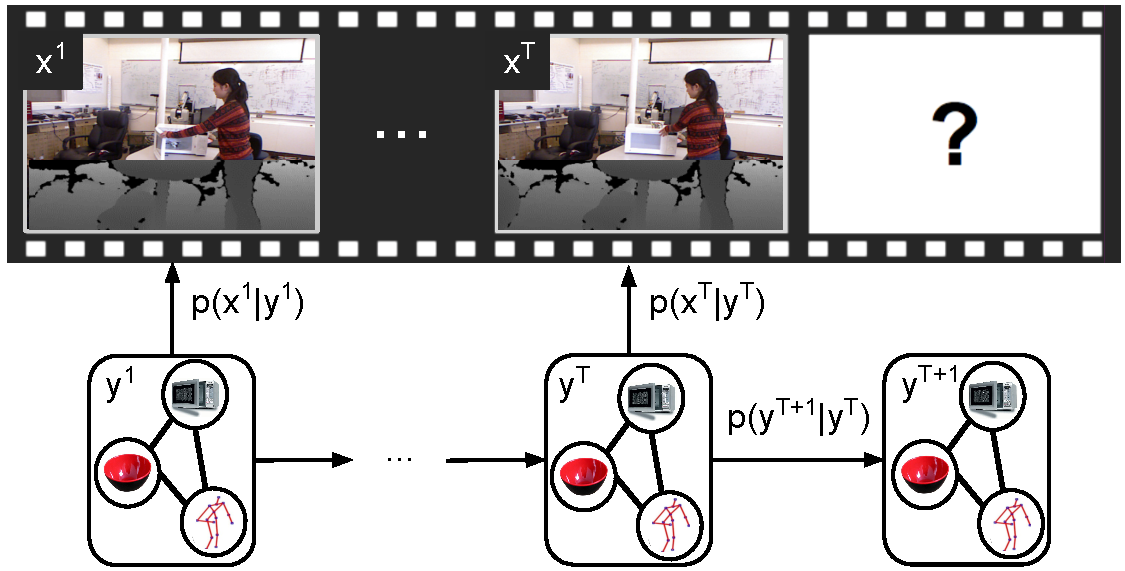
\includegraphics[width=\textwidth]{Fig1}
\caption{Figure is showing the state and measurements at each time represented by a CRF.
Our algorithm, rCRF, enables the application of recursive Bayesian estimation to CRF-based scene models. rCRF computes the full belief over human activity and object affordances ($y^1,\ldots,y^{T+M}$) by using RGB-D Video ($x^1,\ldots,x^T$).}
% In order to so, we propose a new model, rCRF, which can jointly use bayesian filtering and CRFs.}
%  which are not observed.}
%Estimating the belief over a CRF and using the estimated belief for anticipation and robot planning. \emph{(Colors of the nodes are representing the labels.)}}
\label{fig1}
\end{figure}

% modeling temporal evolution is still challenging in such a setting since the sampling procedure does not use temporal information \emph{(see Section~\ref{relwork} for mote details on this challenge)}.
Bayesian filtering methods can accurately estimate a belief (set of probabilities) over variables of interest from sequential data. However, it is still very challenging to estimate a belief over a CRF for two reasons. Firstly, it is not tractable to enumerate the labels over a CRF model since the output space has a dimension exponential in the number of objects, labels, and the temporal length\footnote{Typically with 10 objects, 10 min. length (with 1 sec. long segments), 10 activity and 10 object labels, dimension is $(10^{10}\times10)^{10\times60}=10^{6600}$.}. Secondly, there is a modelling difference between CRFs and Bayesian filtering framework. CRF is based on a discriminative setting whereas the Bayesian filtering mostly relies on the generative formulation.
% that requires the conditional probability of the observation given the variables of interest.
%where it models the conditional probability of the variables of interest given an observation,

In this chapter, we present a recursive algorithm -- Recursive CRF (rCRF) -- which can efficiently estimate a full belief over a CRF-based temporal scene model. rCRF can be seen as an efficient belief estimation method which enables us to use CRF-based scene model in Bayesian filtering. It models the temporal evolution via Bayesian updates and models the measurements in the scene via CRF. In order to use CRFs in such a scenario, we solve two problems. First, we present an approximation to convert the discriminative likelihood of the CRF into a generative measurement equation. Second, we use structured diversity for tractable computation. To the best of our knowledge, rCRF is the only tractable method that can use a CRF-based scene model in a recursive Bayesian filtering.
%Since we define the belief function recursively, we iterate the message propagation and diverse sampling until the convergence.

We apply the rCRF to the problem of activity detection and anticipation from RGB-D data. As a CRF-based scene model, we use the model from \cite{hemaIJRR} which represents the scene as a CRF over human activity and object affordances. We then use the RGB-D video to detect and anticipate activities via rCRF. %We use the rCRF framework in order to anticipate the future activities as well.

Our experiments show that we outperform the state-of-the-art methods for detection and anticipation, and the improvement in the anticipation accuracy is significant. In addition to the improvements in accuracy, we show that our anticipation also improves the computation time and runs near real-time.

%We believe that the presented efficient and accurate estimation of a full belief can be combined with an optimal decision mechanisms (e.g. minimum Bayes risk \cite{decisionTheory,nabbe2007extending}) for better assitive robots.

In summary, the contributions of this work are:
\begin{itemize}
\item  We present Recursive-CRF (rCRF) method that uses the rich modeling power of CRF in
Bayesian filtering setting.
%  allows CRF-based scene models in a Bayesian filtering.
% \item  We present a recursive method in order to estimate the full belief over an rCRF.
\item  We present a structured-diversity based approach to enable tractable computation of the belief.
\item  We apply our rCRF method to the problem of activity detection and anticipation in
RGB-D videos.
%\item  Our experiments show that rCRF significantly outperforms the state-of-the-art methods, both in accuracy and inference time.
\end{itemize}


% !TEX root = ../../ozan_sener_thesis.tex
\section{Related Work on Graphical Models for Robot Perception}
\label{relwork}
%\vspace{\sectionReduceTop}
%\vspace{1mm}
\noindent
{\bf Bayesian Recursive Filtering:}
\label{parf}
Estimating a belief over variables of interest from partial observations is a widely studied problem \cite{thrunBook}. Sequential Monte Carlo (SMC) ---aka \emph{particle filter}--- is typically used to estimate beliefs in high-dimensional cases. SMC methods represent the belief as a set of samples and we refer the reader to \cite{meanFieldBook} for rigorous analysis.

SMC methods are not directly applicable to spaces like CRF since the number of samples required is intractably high. One solution to this problem is the Rao-Blackwellised particle filter \cite{raob}. It uses a partition of the state variables $\bf{y}$ into two set of variables $\bf{y}_1$ and $\bf{y}_2$ such that the variables in one partition $\bf{y}_2$ can be estimated using the partition $\bf{y}_1$. Then Rao-Blackwellised particle filter \cite{raob} estimates the $\bf{y}_1$ via SMC and directly estimates $\bf{y}_2$ using $\bf{y}_1$. However, for our problem, we are not aware of any state decomposition which enables Rao-Blackwellised particle filter. Although there are discrimantive extensions of Bayesian models like recursive least squares\cite{sarkka}, in this chapter we only consider the states represented by CRFs. Moreover, we are not aware of any Bayesian smoothing formulation applied over CRFs.

One tractable application of the SMC framework to the CRF based scene analysis problems is the ATCRF \cite{hemaAnt} model. ATCRF \cite{hemaAnt} uses a set of heuristics to sample the particles. However, ATCRF faces the problem of computational limitations and requires computationally intractable number of samples for anticipation. We follow the Bayesian filtering theory and efficiently estimate the belief.

%\vspace{2mm}
\noindent
{\bf Structured Diversity and Variants of CRFs:}
CRFs are widely used to solve activity analysis problems \cite{siminchi2005,quattoni2007} in a discriminative setting. CRF models the conditional likelihood of the state given the observations, and the MAP solution can be found. Although this setting is powerful, it does not give any information about the belief other than the MAP state.

Other than the MAP solution, it is also tractable to compute the modes of the CRF \cite{divmbest,mbest,mmode}. These modes can be considered as an approximate state space, and the belief can be computed only for them. Indeed, this claim is empirically validated in many problems like parameter learning \cite{mlparam}, empirical MBR \cite{embr} and discrimantive re-ranking \cite{rerank}.

Among the aforementioned approaches, Div-M-Best \cite{divmbest} is a method applicable to the sequential information. \cite{divmbest} starts by dividing the video into a set of frames and computes the diverse-most-likely solutions of each frame independently. Then, it combines the results via the temporal relations. On the contrary, we formulate the problem as recursive Bayesian smoothing and compute the samples based on temporal relations. Formally, given state variables $\mathbf{y}^1,\ldots,\mathbf{y}^T$ and observations $\mathbf{x}^1,\ldots,\mathbf{x}^T$, we directly sample $p(\mathbf{y}^t|\mathbf{x}^1,\ldots,\mathbf{x}^T)$, whereas, \cite{divmbest} samples $p(\mathbf{y}^t|\mathbf{x}^t)$. Since our sampling procedure uses the entire video, our samples are more accurate.

There are variants of CRFs that rely on sequential models as well such as, Dynamic CRF (dCRF) \cite{dcrf}, Infinite Hidden CRF \cite{ihcrf}, Gaussian Process Latent CRF \cite{gpcrf} and Hierarchical Semi-Markov CRF (HSCRF). Although they are applicable to videos, we are not aware of any tractable method to compute a belief over any of the aforementioned graphical model.

DCRF \cite{ddcrf} learns the observation likelihood --$p(\mathbf{x^t}|\mathbf{y^t})$-- by using the low-dimensional nature of the features and follows Bayesian filtering. Since our features have very high-dimension (for $N$ objects, we have $58N+20N^2+103$ dimensional features), DCRF \cite{ddcrf} is not directly applicable. However, it is possible to learn $p(\mathbf{y^t}|\mathbf{x^t})$ and \emph{approximately} use the DCRF formulation by assuming observation and label likelihoods are equal. Moreover, This approach can be shown equivalent to finding local maximum of energy function defined by \cite{hemaIJRR} following the formulation of Fox et al \cite{foxThesis}.

It is also common to compute a belief over latent nodes as in the case of infinte hidden CRF \cite{ihcrf} and Gaussian Process Latent CRF\cite{gpcrf}. However, they are not directly applicable to our problem since they can compute a belief only over the latent node. CRF-Filter \cite{crffilter} is a closely related approach which uses CRFs in a particle filtering scenario. However, it is based on sampling of a low dimensional state space and it is not applicable to our rich model either.

%\vspace{2mm}
\noindent
{\bf Human Activity Detection and Anticipation:} Early works relied solely on human poses. These works range from jointly segmenting and recognizing sub-activities \cite{hoai2011,shi2011} to choosing a relevant model out of activity models \cite{pyry2012}. Main limitation of these methods is that they do not use the object information. Some methods successfully model and use the relations of the human-poses and objects in the scene \cite{davis2009,feifei2010,jiang2012,hall}. However, a significant drawback of these works is missing the fact that object affordance is more important than object types for activities \cite{gibson1979}. Indeed, object affordance based models had higher performance (e.g., \cite{hemaIJRR}). A recent work modelled human activities with latent models \cite{latentIcra} and also handled the disagreements among the activity annotations \cite{rss2014}.

Another drawback of these methods is the requirement of the entire activity. Detecting the activity in its early stages is especially crucial for assistive robotics and surveillance systems. Although a few recent work adress the problem of activity detection with partial/early information \cite{torre2012,ryoo2011}, these works do not perform anticipation. There are a few recent works addressing \emph{what human will perform next} by using trajectory prediction. It is possible to predict the trajectory of the human  using inverse reinforcement learning in 2D \cite{ziebart2009,kuderer2012,kitani2012} or 3D \cite{dragan2012}. However, these models rely on the low-dimensional structure of the 2D/3D coordinate space and therefore they do not apply to rich models like CRF.

Recent work on anticipatory temporal CRF \cite{hemaAnt} considers an anticipation with a CRF model. It anticipates the future via augmenting set of possible future observations to the CRF. It is also extended with an improved human motion model based on a Gaussian process \cite{gpcrf}. However, their accuracy significantly drops for a long anticipation horizon since they fail to represent the uncertainty. Our method overcomes these problems by recursively estimating a full belief.
%\vspace{\sectionReduceBot}


%\input{background}
% \section{Belief over Sub-Activities and Object Affordances}
% !TEX root = robobrain.tex

% \section{Technical Challenges}
\section{Overview}
\label{overviewPaper}

\robobrain{} is a never ending learning system  that  continuously incorporates
new knowledge from  its partner projects and from different Internet sources.
One of the functions of \robobrain{} is to represent the knowledge from various sources as a graph,
as shown in  Figure~\ref{fig:graph}. The nodes of the graph represent concepts and edges represent the
relations between them. The connectivity of the graph is increased through a set of graph operations
that allow additions, deletions and updates to the graph. As of the date of this submission,
\robobrain{} has successfully
connected knowledge from sources like WordNet, ImageNet, Freebase, OpenCyc,
 parts of Wikipedia and other partner projects. These knowledge sources provide lexical knowledge, grounding of concepts into images and common sense facts about the world.

The knowledge from the partner projects and Internet sources can sometimes be erroneous. \robobrain{}
handles inaccuracies in  knowledge by maintaining beliefs over the correctness of the concepts and
relations. These beliefs depend on how much \robobrain{} trusts a given source of knowledge, and also the
feedback it receives from crowd-sourcing (described below). For every incoming knowledge, \robobrain{}
also makes a sequence of decisions on whether to form new nodes, or edges, or both. Since the
knowledge carries semantic meaning \robobrain{} makes many of these decisions based on the
contextual information that it gathers from nearby nodes and edges. For example, \robobrain{} resolves
polysemy using the context associated with nodes. Resolving polysemy is important because a `plant'
could mean a `tree' or an `industrial plant' and merging the nodes together will create errors in the
graph.


\robobrain{} incorporates supervisory signals from humans in the form of crowd-sourcing feedback. This
feedback allows \robobrain{} to update its beliefs over the correctness of the knowledge, and to modify the
graph structure if required. While crowd-sourcing feedback was used in some previous works as
means for data collection (e.g.,~\citep{imagenet2009,Russell08}), in \robobrain{} they serve as supervisory
signals that improve the knowledge engine. \robobrain{} allows user interactions at multiple levels: (i)~
Coarse feedback: these are binary feedback where a user can ``Approve'' or ``Disapprove'' a concept
in \robobrain{} through its online web interface; (ii) Graph feedback: these feedback are elicited on 
\robobrain{} \textit{graph visualizer}, where a user modifies the graph by adding/deleting nodes or edges; (iii)
Robot feedback: these are the physical feedback given by users directly on the robot.

In this paper we discuss different aspects of \robobrain{}, and show how \robobrain{} serves as a knowledge layer for the robots. In order to support knowledge sharing, learning, and crowd-sourcing feedback we develop a large-scale distributed system. We describe the architecture of our  system in Section~\ref{sec:system}. In Section~\ref{sec:raquel} we describe the robot query library, which allow robots to interact with \robobrain{}.  Through experiments we show that robots can use \robobrain{} \textit{as-a-service} and that knowledge sharing through \robobrain{} improves existing robotic applications. We now present a formal definition of our Robot Knowledge Engine and the graph.

% !TEX root = ../../ozan_sener_thesis.tex
\section{Belief Estimation with  rCRF}
\label{theory}
In this section, we develop the Recursive Conditional Random Field (rCRF) to use CRF in a Bayesian filtering setting. rCRF jointly uses rich model of CRF and the recursive nature of the Bayesian filtering to compute an accurate belief. We first define our modelling assumptions in Section~\ref{rcrfdef}, and then we introduce a link between the CRF likelihood and the measurement likelihood in Section~\ref{fromto} in order to compute the posterior belief. In Section~\ref{beliscrf}, we further show that the resulting posterior belief is equivalent to a CRF. Moreover, this equivalence enables efficient computation via the diversity based method \cite{divmbest} developed for CRFs.
\subsection{Recursive Conditional Random Field}
\label{rcrfdef}
Consider a sequential estimation problem in which we are interested in variables $\mathbf{y}^t$ using observations $\mathbf{x}^t$ where $t$ is the temporal variable. In our application, $t$ is the temporal segment id. We note RGB-D camera reading as $\mathbf{x}^t$, and object and activity labels as $\mathbf{y}^t$. We now define the Recursive Conditional Random Field (rCRF) framework for such a problem following the assumptions of Hidden Markov Models.

\begin{mydef}
Let $\mathcal{G}^t=(V^t,E^t)$ be set of graphs indexed by the temporal variable $t$ and $\mathbf{y}^t$ is indexed by the vertices of $\mathcal{G}^t$ as $\mathbf{y}^t=(y^t_v)_{v \in V^t}$. Then, ($\mathbf{x}^{1\ldots T}$,$\mathbf{y}^{1\ldots T}$) is a \textbf{\textit{Recursive Conditional Random Field}} with dynamics $p_v(\cdot|\cdot)$ when

\begin{enumerate}
	\item For each $t$, $(\mathbf{y}^t,\mathbf{x}^t)$ is a CRF over $\mathcal{G}^t=(V^t,E^t)$
%	\item $\mathbf{y^t} \perp \mathbf{y^{t-k}} | {\mathbf{y^{t-1}}} \quad  \forall {k>1}$
\item $p(\mathbf{y}^{t}|\mathbf{y}^{1},\ldots,\mathbf{y}^{t-1}) = p(\mathbf{y}^{t}|\mathbf{y}^{t-1}) \quad  \forall t$ \hfill (Markov)
%\mathbf{y^{t+1}} \perp \mathbf{y^{t-1}} \; | \; {\mathbf{y^{t}}} \quad  \forall t$ \hfill (Markov)
%	\item $\mathbf{y^{t+1}} \perp \mathbf{y^{t-1}} \; | \; {\mathbf{y^{t}}} \quad  \forall t$ \hfill (Markov)
\item $p(\mathbf{x}^t|\mathbf{y}^1,\ldots,\mathbf{y}^t,\mathbf{x}^1,\ldots,\mathbf{x}^{t-1})=p(\mathbf{x}^t|\mathbf{y}^t)\quad  \forall t$ \hfill
%\item $\mathbf{x^t} \perp \mathbf{y^u} | \mathbf{y^t} \quad  \forall {u \neq t}$ \hfill (Measurements are Cond.Ind.)
\item $p(\mathbf{y}^t=\mathbf{y}|\mathbf{y}^{t-1}=\mathbf{y^\prime})=p_v(\mathbf{y}|\mathbf{y^\prime})$ \hfill (stationarity)
\end{enumerate}
$\hfill \blacksquare$
\end{mydef}
\begin{figure}[ht]
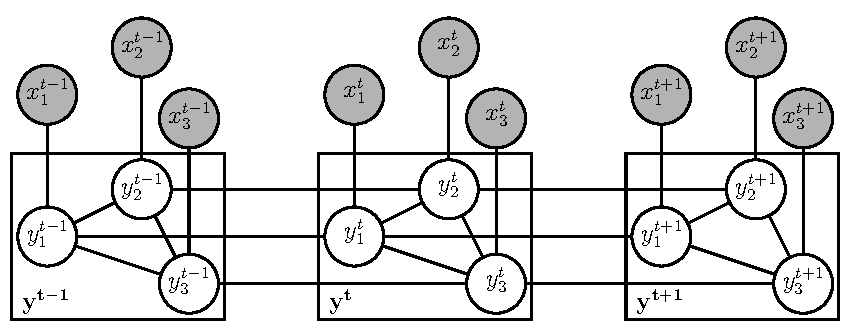
\includegraphics[width=\textwidth]{hmmcrf}
\caption{{\bf rCRF is defined over a temporal CRF.} The graphical model, we use within the rCRF, is a temporal CRF with additional constraints. We impose a special structure through the conditions we state in the definition. For the visualization purposes, we show there nodes per segment although rCRF can handle any number of nodes.}% Shaded nodes represent the observations.
\label{rCrf}
\end{figure}

We visualize the graphical model representation of the rCRF in Figure \ref{rCrf}. In this work, we are interested in the belief over state variables at a given time instant $t$ as:
\begin{equation}
bel^t(\mathbf{y}) = p(\mathbf{y}^t=\mathbf{y}|\mathbf{x}_1,\ldots,\mathbf{x}_T) \label{beldef}
\end{equation}
Here, $T$ denotes the length of the video. Hence, in rCRF the belief of any frame is supported by the entire video. Moreover, the time instant $t$ can be greater than the video length $T$ as well. Hence, rCRF naturally supports anticipation setting.
% This problem is typically referred as Bayesian smoothing.

We then decompose the belief by using the independence properties of the rCRF as:
\begin{equation}
bel^t(\mathbf{y}) \propto  \underbrace{p(\mathbf{y}^t=\mathbf{y}|\mathbf{x}^1,\ldots,\mathbf{x}^t)}_{\alpha^t(\mathbf{y})} \underbrace{p(\mathbf{x}^{t+1},\ldots,\mathbf{x}^T|\mathbf{y}^t=\mathbf{y})}_{\beta^t(\mathbf{y})}
\label{beldec}
\end{equation}
Moreover, $\alpha^t$ and $\beta^t$ can be computed recursively by using forward and backward  messages. Following \cite{hmm},
\begin{equation}
\begin{aligned}
\alpha^t(\mathbf{y}^t) &= p(\mathbf{x}^t|\mathbf{y}^t)\sum_{\mathbf{y}^{t-1}} \alpha^{t-1}(\mathbf{y}^{t-1}) p(\mathbf{y}^{t}|\mathbf{y}^{t-1}) \\
\beta^t(\mathbf{y}^t) &= \sum_{\mathbf{y}^{t+1}} p(\mathbf{x}^{t+1}|\mathbf{y}^{t+1}) \beta^{t+1}(\mathbf{y}^{t+1}) p(\mathbf{y}^{t+1}|\mathbf{y}^{t})
\end{aligned}
\label{mespas}
\end{equation}
\noindent
with initializations $\alpha^1(\mathbf{y}^1)=p(\mathbf{x}^1|\mathbf{y}^1)$ and $\beta^T(\mathbf{y}^T)=1$.

\subsection{Computing the belief using an rCRF}
\label{fromto}
Recursive definition in (\ref{mespas}) has two significant drawbacks:
 firstly, CRF is modelling $p(\mathbf{y}^t|\mathbf{x}^t)$ instead of $p(\mathbf{x}^t|\mathbf{y}^t)$ and the transformation is not trivial. Secondly, computation of the messages require a summation over the entire output space, and it has an exponential dimension. In this section, we first compute the posterior of the observation given labels $p(\mathbf{x}^t|\mathbf{y}^t)$ by using the CRF posterior likelihood $p(\mathbf{y}^t|\mathbf{x}^t)$. Then, we show that the belief function at time $t$, $bel^t(\mathbf{y})$, can be approximately represented as a Gibbs measure over $\mathcal{G}^t$. Then, we conclude that the belief, $bel^t(\mathbf{y})$, is a CRF over the graph $\mathcal{G}^t$ with modified energy functions.
%Finally, we suggest a method to efficiently represent the belief over small number of samples in section \ref{divm}.
\subsubsection{From $p(\mathbf{y}^t|\mathbf{x}^t)$ to $p(\mathbf{x}^t|\mathbf{y}^t)$}
Since $(\mathbf{x}^t,\mathbf{y}^t)$ is a CRF, the posterior of the label given the observation follows \cite{geman}; %a Gibbs measure \cite{geman} as;
\begin{equation}
p(\mathbf{y}^t|\mathbf{x}^t) \propto \exp\left( \sum_{i \in V^t} \theta_{x^t_i}(y^t_i) + \sum_{i,j \in E^t} \theta_{x^t_i,x^t_j}(y^t_i,y^t_j)  \right)
\label{crflogl}
\end{equation}
where $\theta$ is the energy function defined over the node set \mbox{$v \in V^t$ }as $\theta_{v}$ and over the edge set \mbox{$(u,v) \in E^t$} as $\theta_{u,v}$.

%\frac{p(\mathbf{y}^t|\mathbf{x}^t)}{p(\mathbf{y}^t)} =
In order to transform  $p(\mathbf{y}^t|\mathbf{x}^t)$ into  $p(\mathbf{x}^t|\mathbf{y}^t)$, we use Bayes rule;
$p(\mathbf{x}^t|\mathbf{y}^t) \propto  \frac{p(\mathbf{y}^t|\mathbf{x}^t)}{ \sum_{x^t} p(\mathbf{y}^t|\mathbf{x}^t)p(\mathbf{x}^t)}$ and compute $p(\mathbf{y}^t)$ as; %the denominator as;
\begin{equation}
p(\mathbf{y}^t)=\sum_{\mathbf{x}^t} \exp\left( \sum_{i \in V^t} \theta_{x^t_i}(y^t_i) + \sum_{i,j \in E^t} \theta_{x^t_i,x^t_j}(y^t_i,y^t_j) \right) p(\mathbf{x}^t)
\end{equation}
For tractability, we approximate the $p(\mathbf{y}^t)$ with its lower bound after applying the Jensen inequality as;
\begin{equation}
	\small
p(\mathbf{y}^t) \approx \exp ( \sum_{i \in V^t} \underbrace{\sum_{\mathbf{x}^t} \theta_{x^t_i}(y^t_i)  p(\mathbf{x}^t)}_{\tilde{\theta}(y^t_i)} + \sum_{i,j \in E^t} \underbrace{ \sum_{\mathbf{x}^t}  \theta_{x^t_i,x^t_j}(y^t_i,y^t_j) p(\mathbf{x}^t)}_{\tilde{\theta}(y^t_i,y^t_j)} )
\end{equation}

% \todo{
We then estimate the inner summations $\tilde{\theta}(\cdot)$
% , expectation over $\mathbf{x}$, )
% empirically by
from the training data
% In other words, we
using Monte Carlo method
% to compute inner summations
 as \mbox{$\tilde{\theta}(\cdot) = \frac{1}{N}\sum_{i=1}^N \theta_{\mathbf{x}^{(i)}}(\cdot)$} where $N$ is the number of training samples and $\mathbf{x}^{(i)}$ is the $i^{th}$ training sample.
 %  with abuse of notation.
 Therefore, we can compute the observation likelihood as:  $p(\mathbf{x}^t|\mathbf{y}^t) \propto$
\begin{equation}\small
\exp\left( \sum_{i \in V^t} \theta_{x^t_i}(y^t_i) - \tilde{\theta}(y^t_i) + \sum_{i,j \in E^t} \theta_{x^t_i,x^t_j}(y^t_i,y^t_j) - \tilde{\theta}(y^t_i,y^t_j)  \right)
\label{obsprob}
\end{equation}

\subsubsection{Belief is a CRF}
\label{beliscrf}
Here we compute the belief (\ref{beldec}) in terms of forward and backward messages and CRF likelihood. We then show that the posterior belief is a CRF. This observation enables us to use efficient methods developed for CRFs.

In order to compute the belief (\ref{beldec}), we decompose
% assume that
% start with the simplifying assumption that
the system dynamics using the independence assumption in the graph in Fig.~\ref{rCrf}.
This gives us \mbox{$p(\mathbf{y}^t|\mathbf{y}^{t-1})=\prod_{i} p(y^t_i|y^{t-1}_i)$}.
% In other words, the system dynamics model does not model correlations
%
% we model the relationship between variables via CRF and do not consider them while modelling temporal dynamics.
%
%After decomposing the state transition dynamics,
We then compute the belief function as \mbox{$bel(\mathbf{y}^t)=\alpha^t(\mathbf{y}^t)\beta^t(\mathbf{y}^t)$} by using equations (\ref{mespas}) and (\ref{obsprob}). After algebraic manipulations, the belief function can be approximated as follows (see supplementary material for a detailed derivation):
\iffalse
\begin{equation}\small
	\begin{aligned}
&bel(\mathbf{y}^t) \propto \exp\left[  \sum_{i,j \in E^t} \left( \theta_{x^t_i,x^t_j}(y^t_i,y^t_j) - \tilde{\theta}(y^t_i,y^t_j) \right) \right. \\
&\left. \sum_{i \in V^t} \left( \theta_{x^t_i}(y^t_i) - \tilde{\theta}(y^t_i) +  \sum_{\mathbf{y^{t-1}}} \alpha^{t-1}(\mathbf{y}^{t-1}) \log p(y^t_i|y^{t-1}_i) \right. \right. \\
&+\left.\left.\sum_{\mathbf{y}^{t+1}} \beta^{t+1}(\mathbf{y}^{t+1}) p(\mathbf{x}^{t+1}|\mathbf{y}^{t+1}) \log p(y^t_i|y^{t-1}_i) \right) \right]
\end{aligned}
\label{crfbelief}
\end{equation}
\fi

\begin{equation}\small
  \begin{aligned}
&bel(\mathbf{y}^t) \propto \exp\left[  \sum_{i,j \in E^t} \left( \theta_{x^t_i,x^t_j}(y^t_i,y^t_j) - \tilde{\theta}(y^t_i,y^t_j) \right) \right. \\
&\left. \sum_{i \in V^t} \left( \theta_{x^t_i}(y^t_i) - \tilde{\theta}(y^t_i) +  \sum_{\mathbf{y}^{t-1}} \alpha^{t-1}(\mathbf{y}^{t-1}) \log p(y^t_i|y^{t-1}_i) \right. \right. \\
&+\left.\left.\frac{1}{\gamma}\sum_{\mathbf{y}^{t+1}} \beta^{t+1}(\mathbf{y}^{t+1}) p(\mathbf{x}^{t+1}|\mathbf{y}^{t+1}) \log p(y^{t+1}_i|y^{t}_i) \right) \right]
\end{aligned}
\label{crfbelief}
\end{equation}
where $\gamma=\sum_{\mathbf{y}^{t+1}} \beta^{t+1}(\mathbf{y}^{t+1}) p(\mathbf{x}^{t+1}|\mathbf{y}^{t+1})$

One property to observe is the decomposition of the belief over the graph. Resulting belief function, (\ref{crfbelief}), is a summation over energy terms defined over nodes $i \in V^t$ and edges $i,j\in E^t$. Hence, belief $bel^t(\cdot)$ is a Gibbs measure over $\mathcal{G}^t$. By using Hammersley-Clifford theorem \cite{hc1971}, we  conclude that the posterior belief in rCRF is also a CRF. In other words, belief is a CRF defined over the same graph with a modified energy.

\subsubsection{Belief via Diverse-Most-Likely Samples}
\label{divm}
Since we computed the belief function and showed that it is equivalent to a CRF, we now need
an efficient method for computing it.

% here we use an existing method, computing diverse-most-likely samples \cite{divmbest}, that is developed for a CRF, in order to efficiently compute the belief.

We follow the observation that CRF-likelihood over a natural scene concentrates on a few diverse samples \cite{divmbest} because each scene only has a few plausible explanation. So, we compute the belief for only those samples. In other words, let's assume the set of all plausible solutions at time $t$ is $\mathbf{Y}^t={\mathbf{y}^{t,1},\ldots,\mathbf{y}^{t,M}}$ where $\mathbf{y}^{t,i}$ is the $i^{th}$ sample at time $t$. We then redefine the belief as;

\begin{equation}
	\text{approx\_bel}^t(\mathbf{y})=\left\{ \begin{array}{cc} \frac{bel^t(\mathbf{y})}{\sum_{\mathbf{y}^\prime \in \mathbf{Y}^t} bel^t(\mathbf{y}^\prime)} & \text{if $\mathbf{y} \in \mathbf{Y}^t$} \\ 0 & \text{o.w.} \end{array} \right.
\end{equation}

Since there are only a few plausible explanation of a visual observation and CRF-based belief concentrates only on those samples, proper selection of the samples $\mathbf{Y}^t$ is expected to work well in practice. These samples are typically selected as the diverse-most-likely solutions of the CRF. They are most-likely samples because we are only interested in the plausible explanations. They are diverse because we are interested in the modes of the CRF other than set of samples around the MAP solution. Diversity is achieved via asserting samples to be at least $\delta$ unit apart from each other via the distance function $\Delta$ (we use hamming distance as a in our experiments). In other words, we solve the following optimization problem in order to get the samples which represent the belief;
\begin{equation}
\begin{aligned}
\mathbf{y}^{t,i} &= \argmax_{\mathbf{y}}  bel^t(\mathbf{y}) \\
&s.t.\,\, \Delta(\mathbf{y},\mathbf{y}^{t,j}) \geq \delta \quad \forall \; {j < i}
\end{aligned}
\label{divopt}
\end{equation}
%where $\bf{y}^{t,i}$ is the $i^{th}$ sample in the $t^{th}$ frame.
This optimization is NP-hard in general; however, since we already showed $bel^t(\bf{y})$ is CRF, we use the existing diverse-m-best algorithms developed for CRFs. We use the Lagrange relaxation by Batra et al. \cite{divmbest}. We explain the details of solving this problem by using \cite{divmbest} in supplementary material.

In summary, we first compute the belief via (\ref{crfbelief}) for all frames by using samples of the previous and the next frame as well as CRF likelihoods. Then, we compute the diverse samples of (\ref{crfbelief}) by using \cite{divmbest}. After computing the samples, we compute the messages $\alpha^t$ and $\beta^t$ by using the equations (\ref{obsprob}) and (\ref{mespas}). We continue to re-sample the beliefs and re-compute the messages recursively until the convergence. Moreover, during the initialization, we only sample the observation function (\ref{obsprob}) since the messages are not available.

% !TEX root = anticipation_divmrf.tex
\section{Human Activity Detection and Anticipation}
\label{rgbd}
In this section, we describe how we apply the rCRF framework to RGB-D videos for human activity detection and anticipation. We are interested in activities such as \emph{reaching} and \emph{moving}, and object affordances such as \emph{reachable} and \emph{movable} as explained in Section~\ref{overview}. We follow the approach in \cite{hemaIJRR}, and start with temporally segmenting the video. This step can be considered as an oversegmentation in the temporal domain. It decreases the computation complexity and enables using motion information as an observation.

We then obtain the observations $\mathbf{x}^t=(L_1^t,L_2^t,H^t)$, by detecting the objects in the first frame and then tracking them. We obtain the human pose $H^t$ through a skeleton tracker. We consider affordances and activities as state \mbox{$\mathbf{y}^t=(O^t_1,\ldots,O^t_N,A)$} where $N$ is the number of objects. We extracted set of features from the observations following the feature functions in \cite{hemaIJRR} (\emph{eg.} relative and absolute location of objects, human joints and their temporal displacements). After extracting the features, we define our CRF as a log-linear CRF and learn the energy function defined in (\ref{crflogl}) by using the Structural SVM \cite{ssvm} as in the case of \cite{hemaIJRR}. We use the first order statistics for temporal dynamics as \mbox{$p_v(y,y^\prime)=p(Y^t_v=y|Y^{t-1}_v=y^\prime)=\frac{\#(Y^t_v=y,Y^{t-1}_v=y^\prime)}{\#(Y^t_v=y\prime)}$} where $\#(\cdot,\cdot)$ is number of the co-occurrence in training data.

After defining the observation, state and dynamics, we apply the rCRF framework. We also summarize the activity detection and anticipation application in Algorithm~\ref{alg:recursive}.%\vspace{-5mm}

\setlength{\textfloatsep}{0.1pt}
\begin{algorithm}
\caption{Compute belief the over $(O^t_{1\ldots N},A^t)$ for \mbox{$t \in [1,T+\tau]$} in an RGB-D Video of length $T$}
\label{alg:recursive}
\begin{algorithmic}
\STATE {\bf Initialization:}
\STATE Compute $L^t_1,\ldots,L^t_N$, and $H^t$ for $t \in [1,T]$ via \cite{hemaIJRR}.
\STATE Compute $p(L^t_{1\ldots N},H^t|O^t_{1\ldots N},A^t)$ for $t \in [1,T]$ via (\ref{obsprob})
\STATE Compute the belief via (\ref{crfbelief}) w/o messages ($\alpha=1,\beta=1$)
\end{algorithmic}
\begin{algorithmic}
\STATE {\bf Detection:}
\REPEAT
\FOR {$t \in [1,T]$}
%\STATE Compute $p(L^t_{1\ldots K},H^t|O^t_{1\ldots K},A^t)$ via (\ref{obsprob})
\STATE Compute the forward/backward messages via (\ref{mespas})
\STATE Compute the belief via (\ref{crfbelief}) an sample via (\ref{divopt})
%\STATE Sample the posterior belief via (\ref{divopt})
\ENDFOR
\UNTIL convergence or number of iterations limit
\STATE {\bf Anticipation:}
\FOR {$t \in [T+1,T+\tau]$}
\STATE Compute only the forward messages via (\ref{mespas})
\STATE Sample the belief directly from the forward messages.
\ENDFOR
\end{algorithmic}
\end{algorithm}

%\vspace{-3mm}
%During the initialization stage in Algorithm~\ref{alg:recursive}, we compute the belief without messages since the recursive computation of the messages requires a belief. After the initialization, we apply the full rCRF algorithm recursively.

Moreover, since the temporal relations are modeled as causal, we do not compute the backward messages during the anticipation. In anticipation, there is also no future observation. Hence, the belief is defined solely by the forward messages. In order to compute the belief for future frames, we propagate the estimated belief. We propagate the belief to the next frame by sampling the next state of the each sample in the belief of the current frame via the temporal dynamics. Then, we choose diverse most likely samples out of the propagated samples via solving (\ref{divopt}) with exhaustive search.

% !TEX root = rCRF.tex
\section{Experimental Results}
In order to experimentally evaluate the proposed rCRF model and the belief computation, we perform experiments on two applications. Firstly, we estimate a belief over the activity a human is performing and the affordances of the objects in the scene by using the RGB-D video. After computing the belief, we detect the most likely activity and affordance sequences and study the improvement in the detection accuracy. Secondly, we test the accuracy of the beliefs in the anticipation setting. Indeed, we show that it is possible to obtain high-quality detection and anticipation via rCRF.

\begin{figure}[ht]
\small
%\begin{singlespace}
\begin{tabular}{p{5mm}@{}l}
\begin{tabular}{r}
\rotatebox[origin=r]{90}{\;\;\;\;\;\;\;Middle Frame}\\
\rotatebox[origin=l]{90}{Belief\;\;\;\;\;\;\;}
\end{tabular}
&
\begin{tabular}{p{3.7cm}p{3.7cm}p{3.7cm}p{3.7cm}}
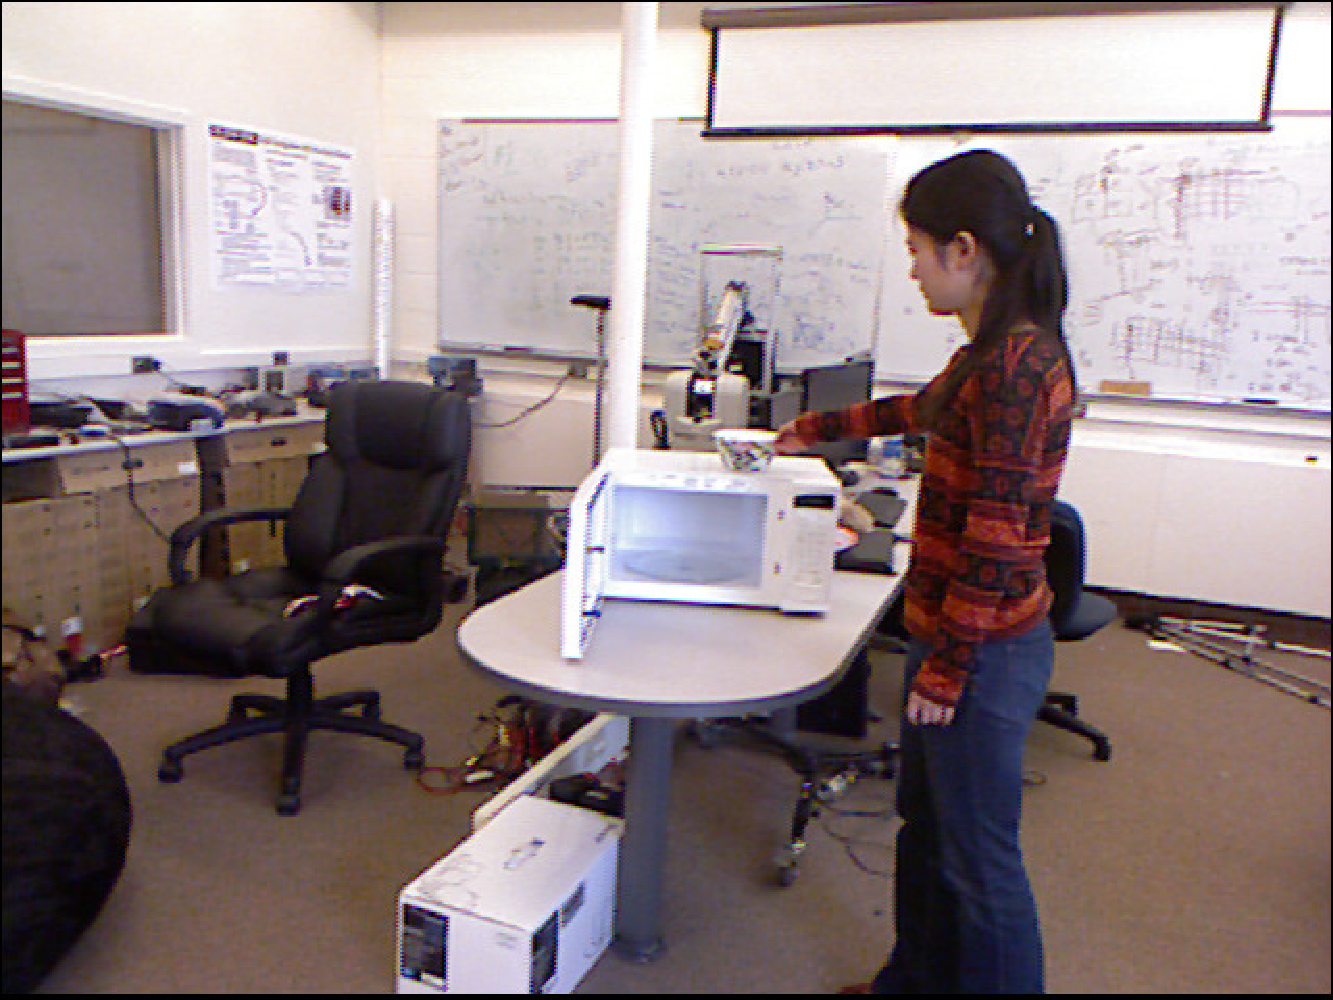
\includegraphics[width=0.225\textwidth]{f10} &
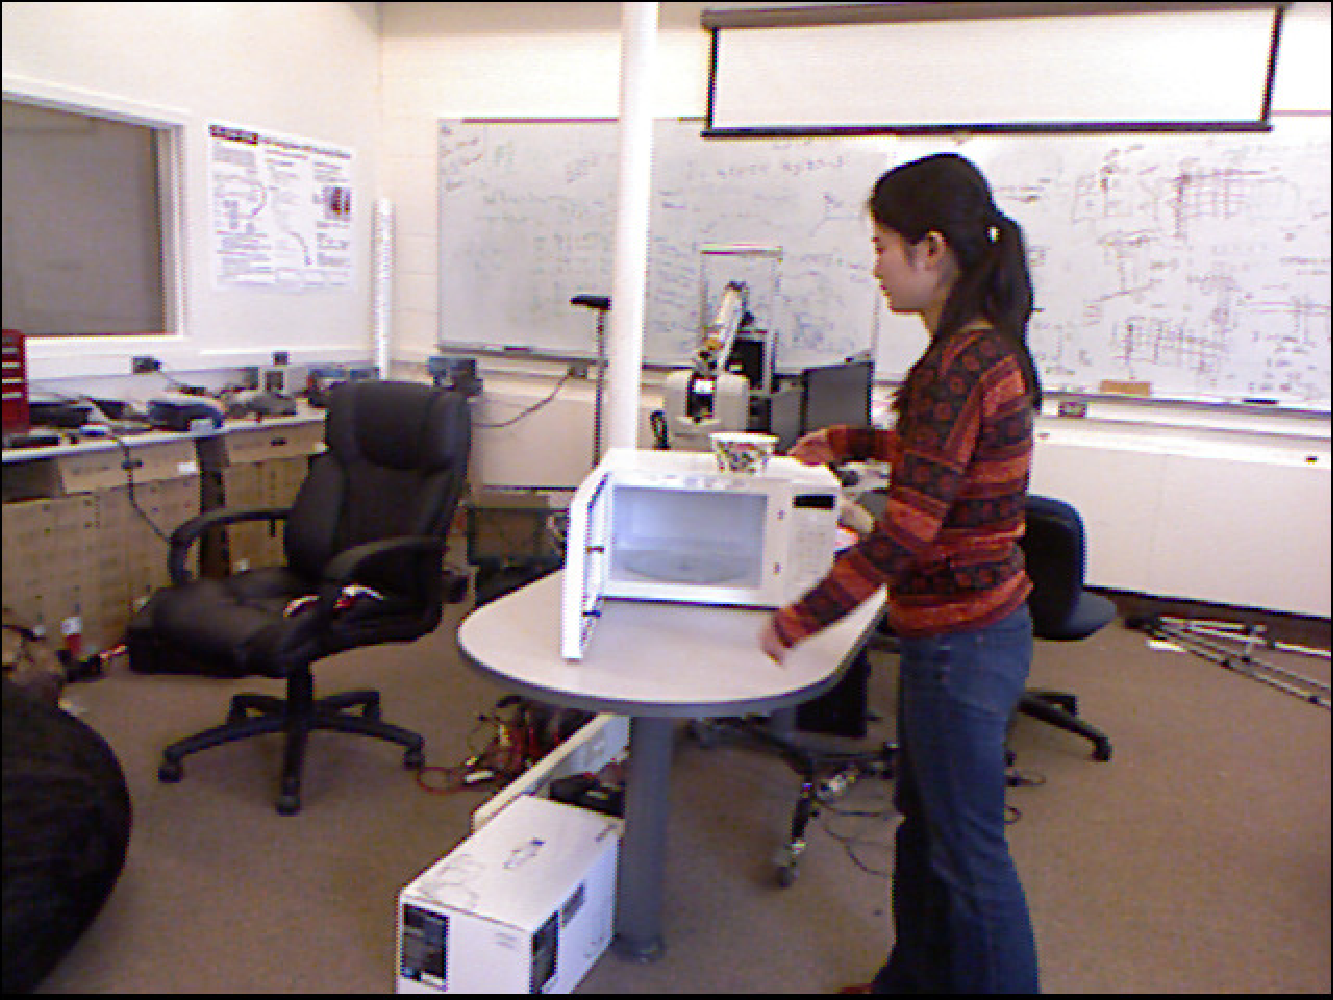
\includegraphics[width=0.225\textwidth]{f11} &
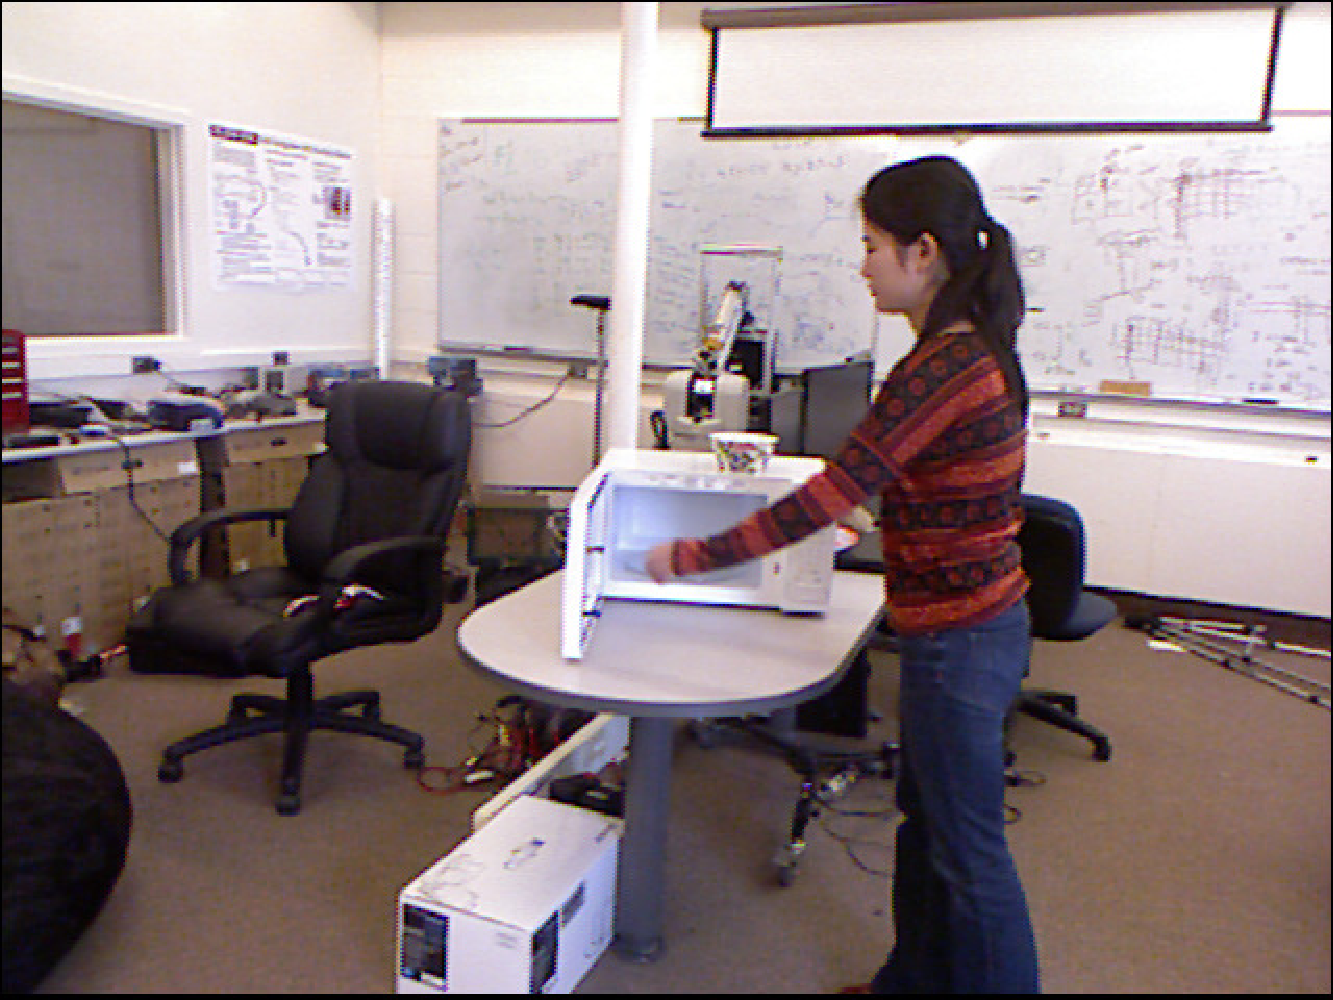
\includegraphics[width=0.225\textwidth]{f12} &
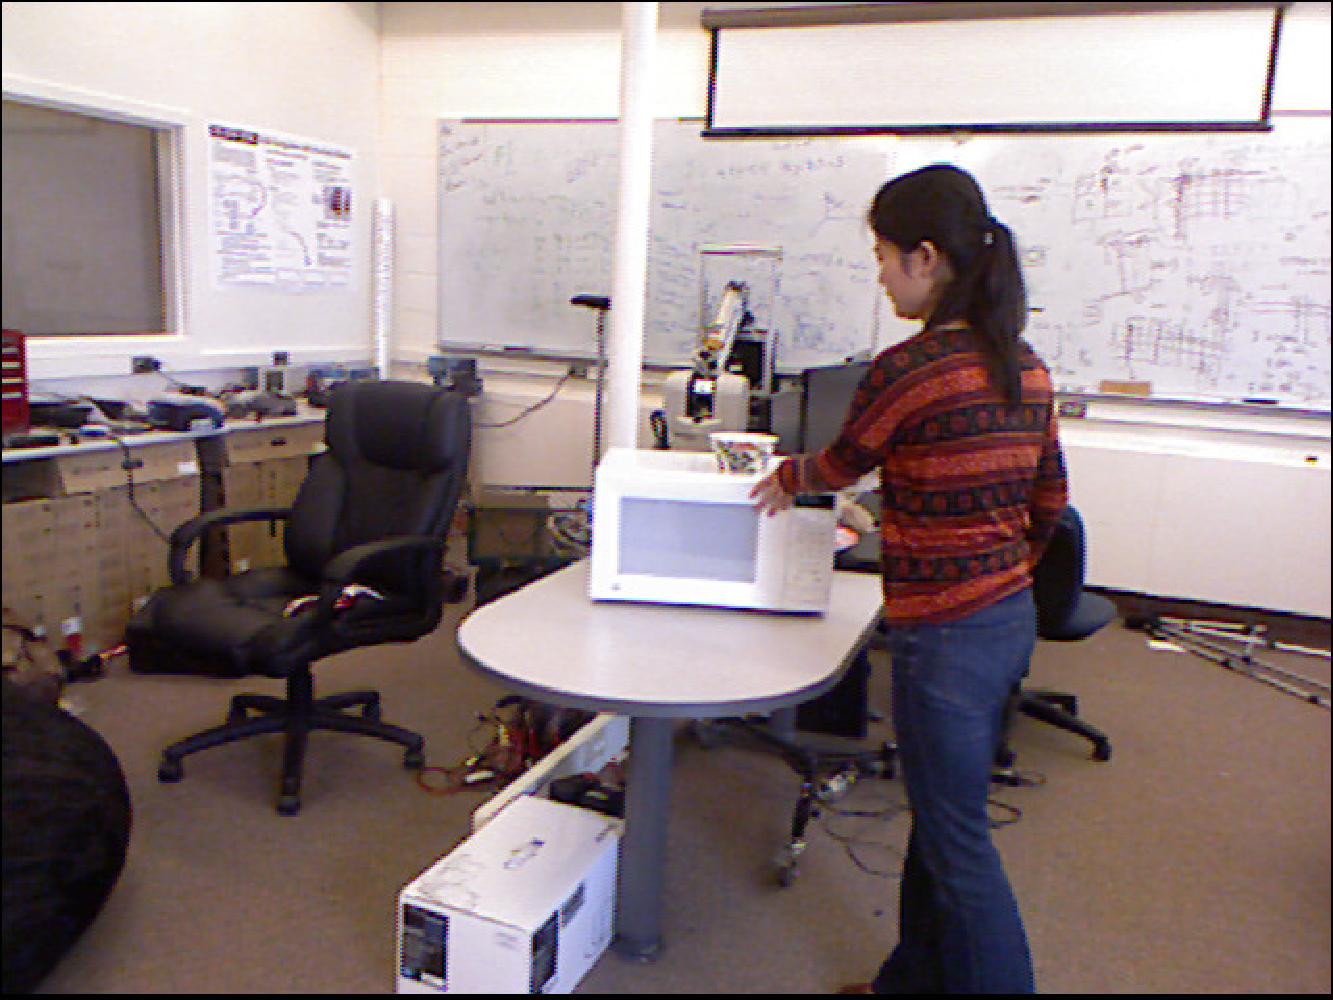
\includegraphics[width=0.225\textwidth]{f13}  \\ %\\%\begin{tabular}{p{3.6cm}p{3.6cm}p{3.6cm}p{3.6cm}}
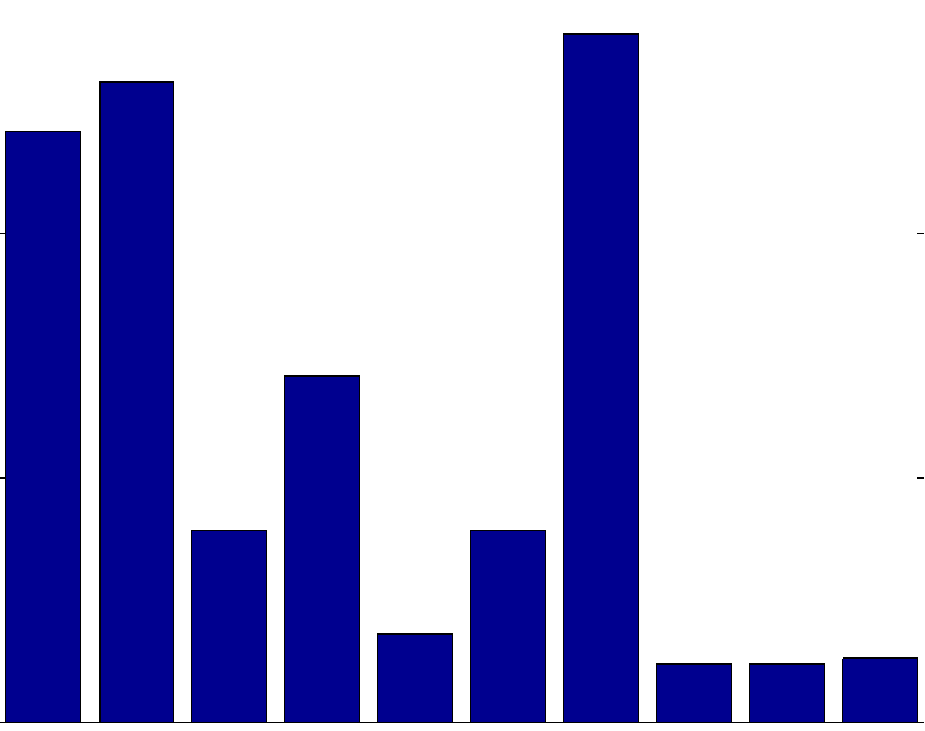
\includegraphics[width=0.225\textwidth, height=8mm]{P10} &
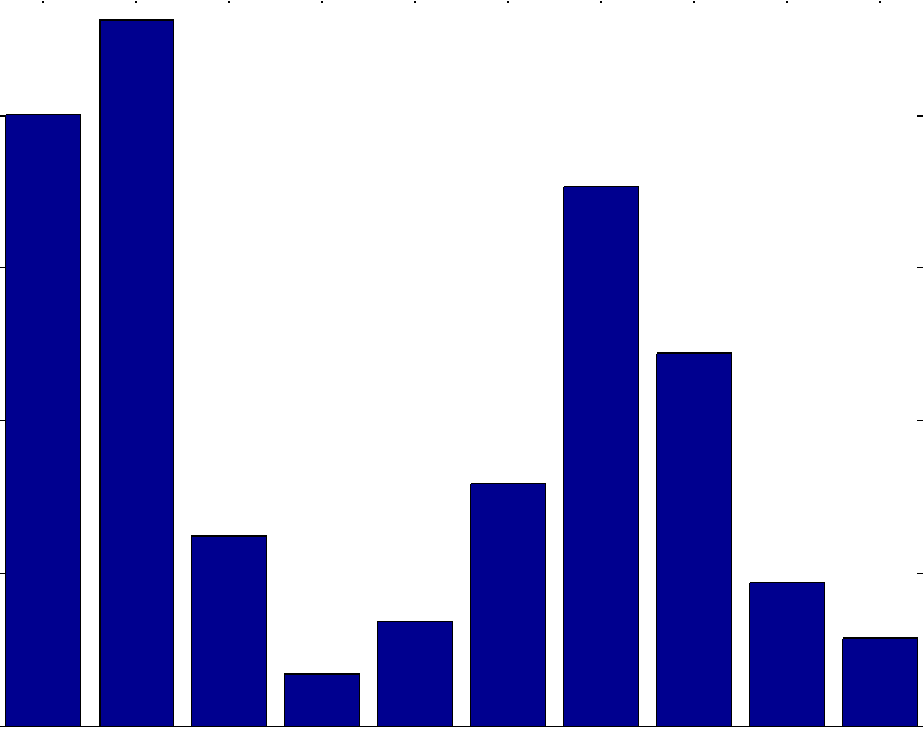
\includegraphics[width=0.225\textwidth, height=8mm]{P12P} &
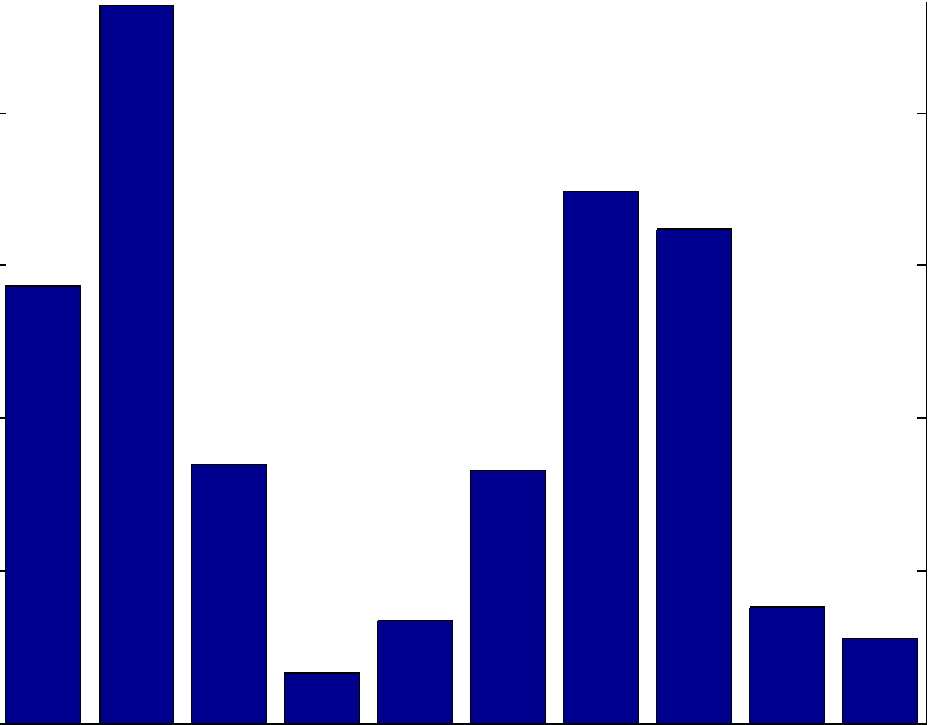
\includegraphics[width=0.225\textwidth, height=8mm]{P13P} &
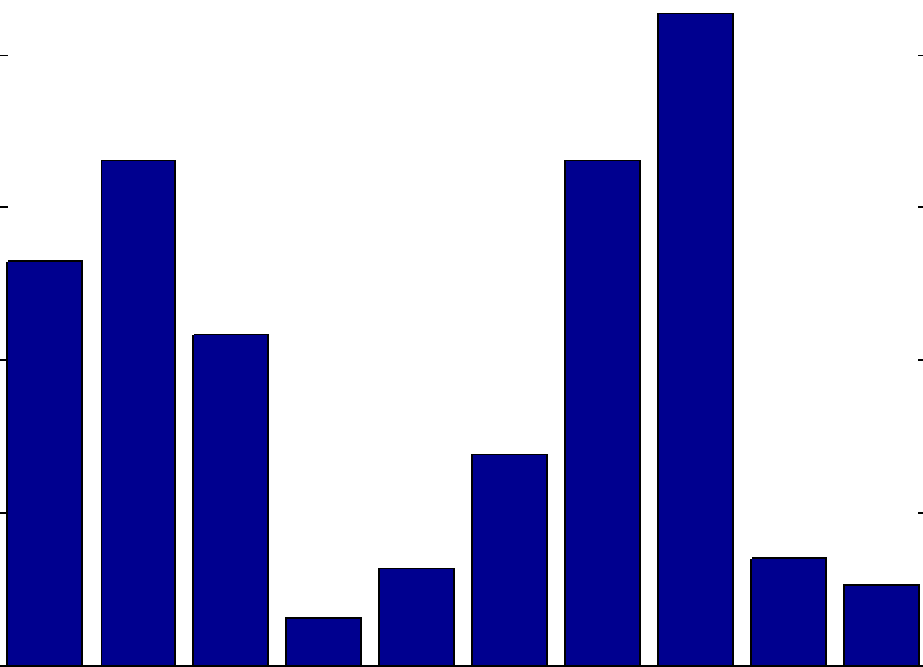
\includegraphics[width=0.225\textwidth, height=8mm]{P14P}  \\

\vspace{-6mm}\hspace{-1mm}\scalebox{0.84}{
\rotatebox[origin=r]{90}{reaching}\hspace{1mm}
\rotatebox[origin=r]{90}{moving}\hspace{1mm}
\rotatebox[origin=r]{90}{pouring}\hspace{1mm}
\rotatebox[origin=r]{90}{eating}\hspace{1mm}
\rotatebox[origin=r]{90}{drinking}\hspace{1mm}
\rotatebox[origin=r]{90}{opening}\hspace{1mm}
\rotatebox[origin=r]{90}{placing}\hspace{1mm}
\rotatebox[origin=r]{90}{closing}\hspace{1mm}
\rotatebox[origin=r]{90}{null}\hspace{1mm}
\rotatebox[origin=r]{90}{cleaning}}&
\vspace{-6mm}\hspace{-1mm}\scalebox{0.84}{
\rotatebox[origin=r]{90}{reaching}\hspace{1mm}
\rotatebox[origin=r]{90}{moving}\hspace{1mm}
\rotatebox[origin=r]{90}{pouring}\hspace{1mm}
\rotatebox[origin=r]{90}{eating}\hspace{1mm}
\rotatebox[origin=r]{90}{drinking}\hspace{1mm}
\rotatebox[origin=r]{90}{opening}\hspace{1mm}
\rotatebox[origin=r]{90}{placing}\hspace{1mm}
\rotatebox[origin=r]{90}{closing}\hspace{1mm}
\rotatebox[origin=r]{90}{null}\hspace{1mm}
\rotatebox[origin=r]{90}{cleaning}}&
\vspace{-6mm}\hspace{-1mm}\scalebox{0.84}{
\rotatebox[origin=r]{90}{reaching}\hspace{1mm}
\rotatebox[origin=r]{90}{moving}\hspace{1mm}
\rotatebox[origin=r]{90}{pouring}\hspace{1mm}
\rotatebox[origin=r]{90}{eating}\hspace{1mm}
\rotatebox[origin=r]{90}{drinking}\hspace{1mm}
\rotatebox[origin=r]{90}{opening}\hspace{1mm}
\rotatebox[origin=r]{90}{placing}\hspace{1mm}
\rotatebox[origin=r]{90}{closing}\hspace{1mm}
\rotatebox[origin=r]{90}{null}\hspace{1mm}
\rotatebox[origin=r]{90}{cleaning}}&
\vspace{-6mm}\hspace{-1mm}\scalebox{0.84}{
\rotatebox[origin=r]{90}{reaching}\hspace{1mm}
\rotatebox[origin=r]{90}{moving}\hspace{1mm}
\rotatebox[origin=r]{90}{pouring}\hspace{1mm}
\rotatebox[origin=r]{90}{eating}\hspace{1mm}
\rotatebox[origin=r]{90}{drinking}\hspace{1mm}
\rotatebox[origin=r]{90}{opening}\hspace{1mm}
\rotatebox[origin=r]{90}{placing}\hspace{1mm}
\rotatebox[origin=r]{90}{closing}\hspace{1mm}
\rotatebox[origin=r]{90}{null}\hspace{1mm}
\rotatebox[origin=r]{90}{cleaning}}
\end{tabular}
\end{tabular}

\begin{tabular}{p{5mm}@{}l}
\begin{tabular}{r}
\rotatebox[origin=r]{90}{\;\;\;\;\;\;\;Middle Frame}\\
\rotatebox[origin=l]{90}{Belief\;\;\;\;\;\;\;}
\end{tabular}
&
\begin{tabular}{p{3.7cm}p{3.7cm}p{3.7cm}p{3.7cm}}
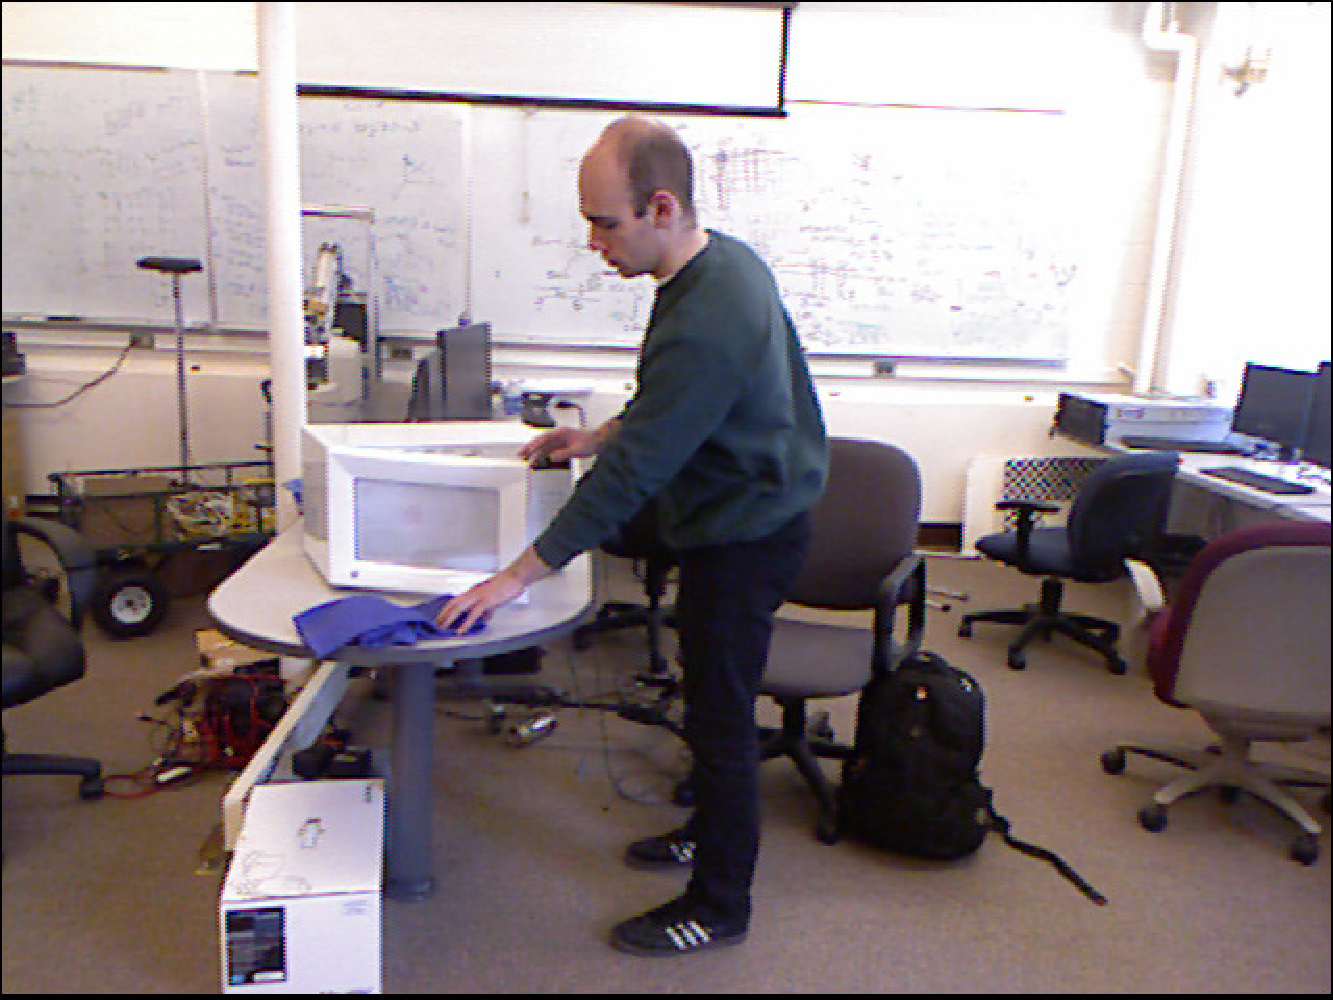
\includegraphics[width=0.225\textwidth]{l5} &
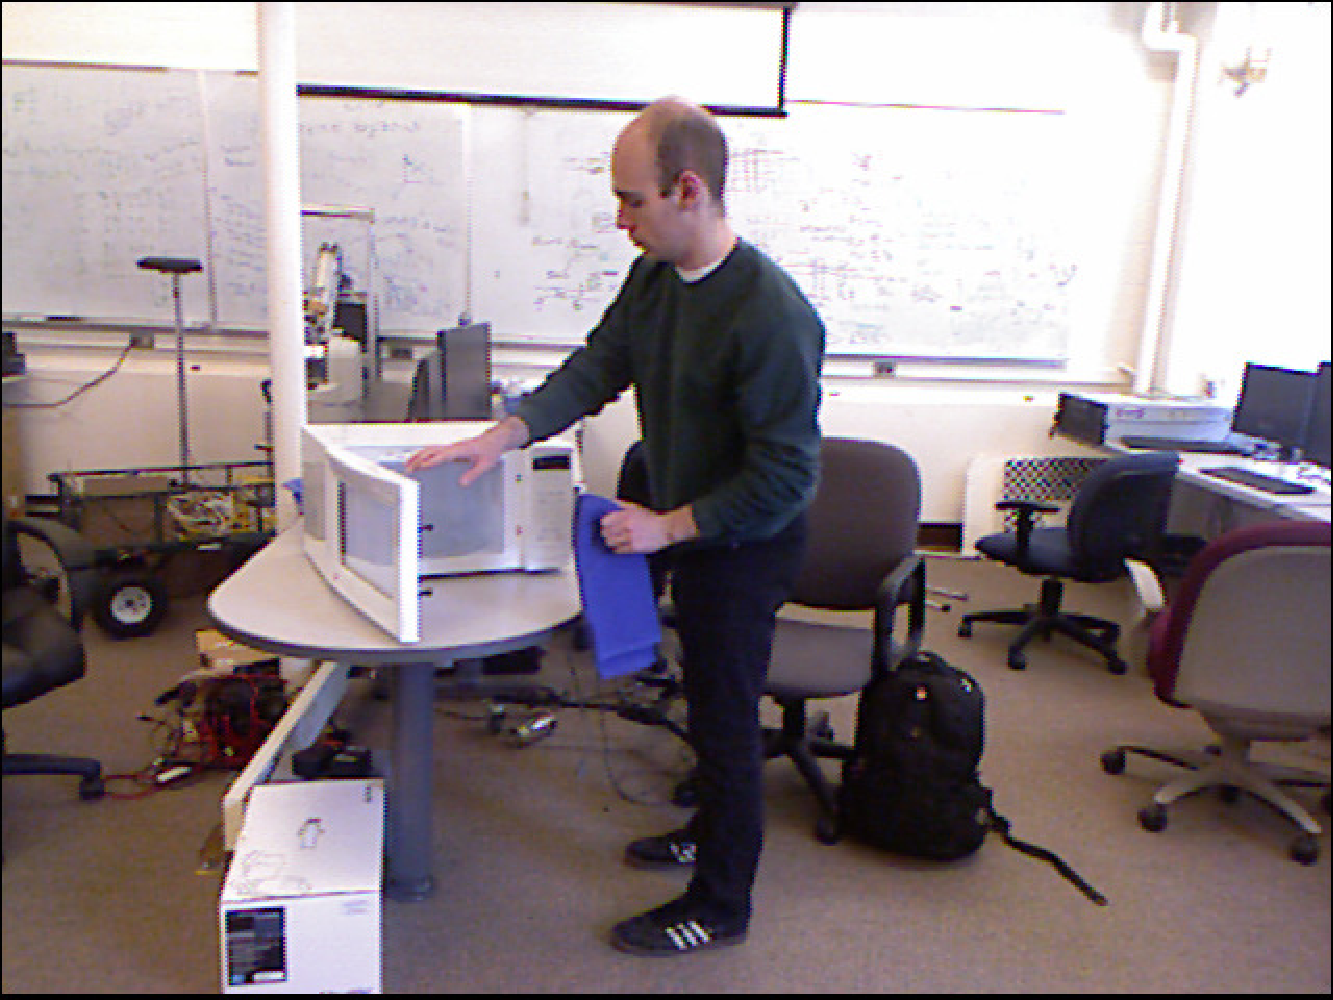
\includegraphics[width=0.225\textwidth]{l6} &
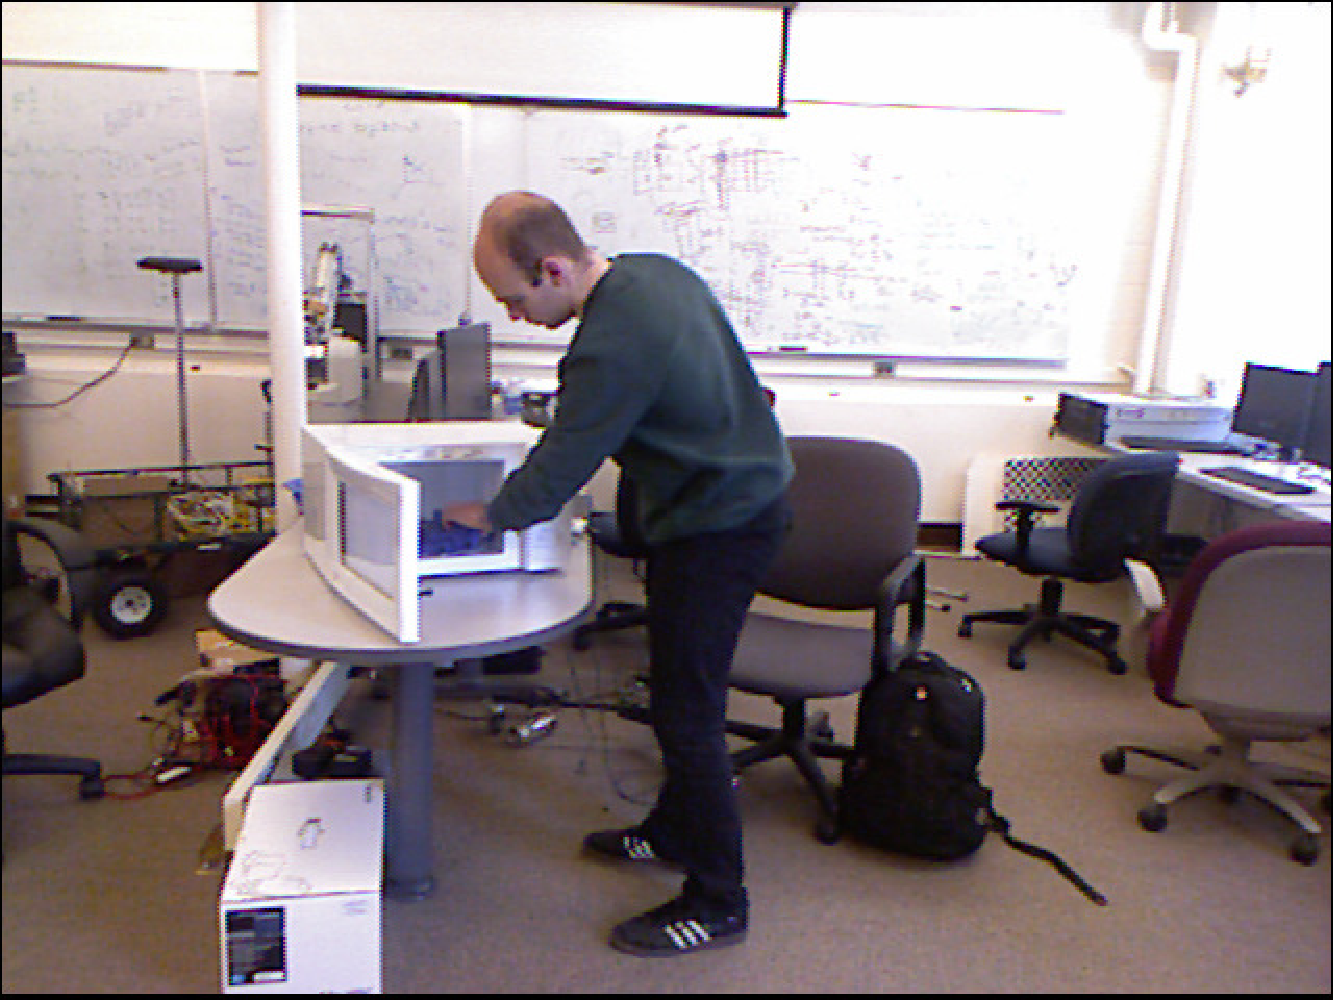
\includegraphics[width=0.225\textwidth]{l7} &
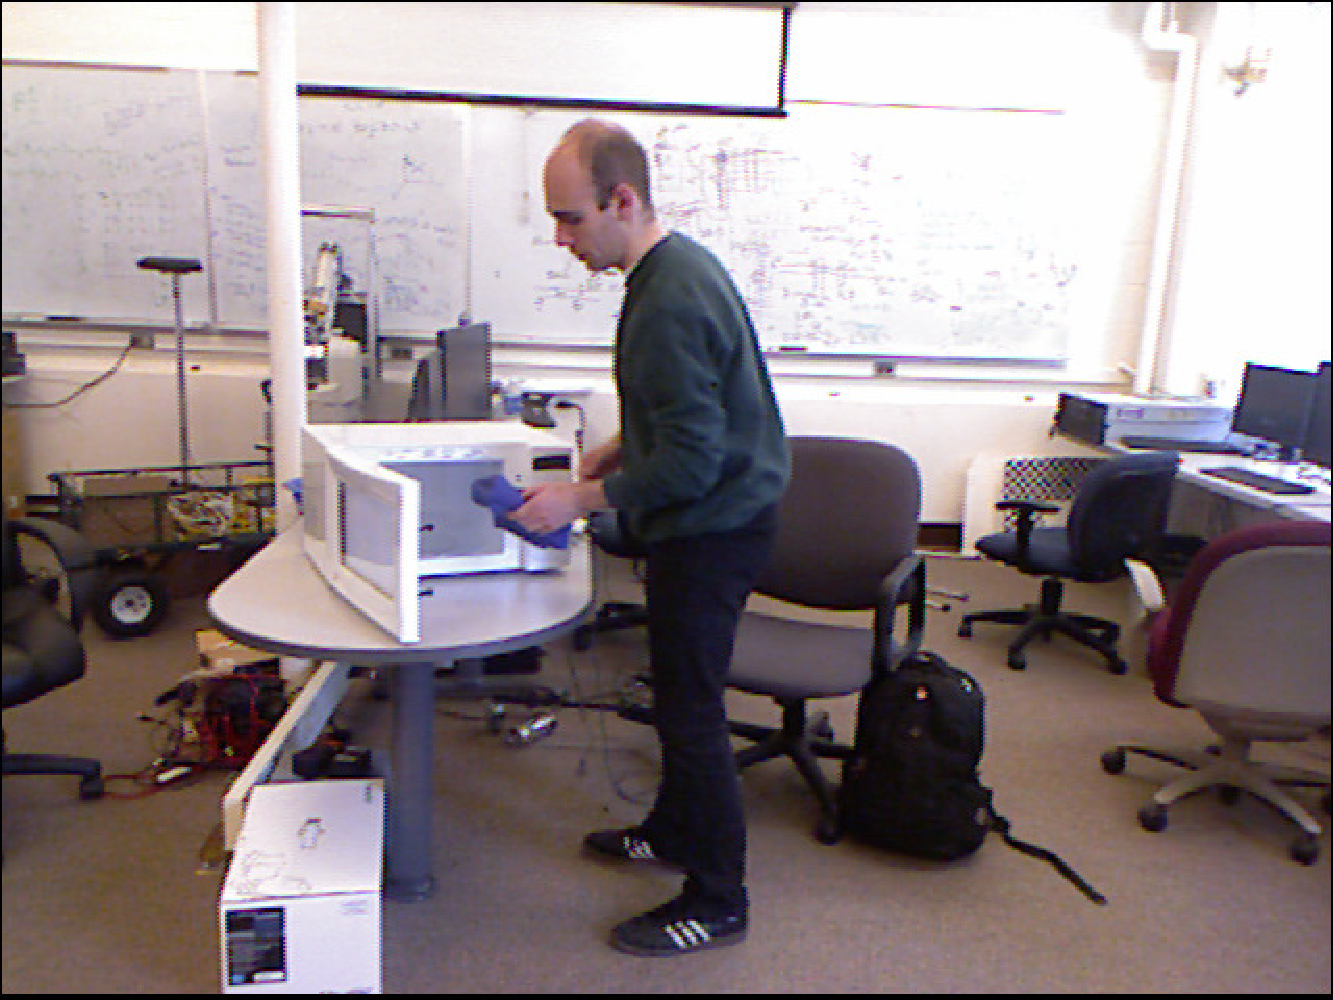
\includegraphics[width=0.225\textwidth]{l8}  \\
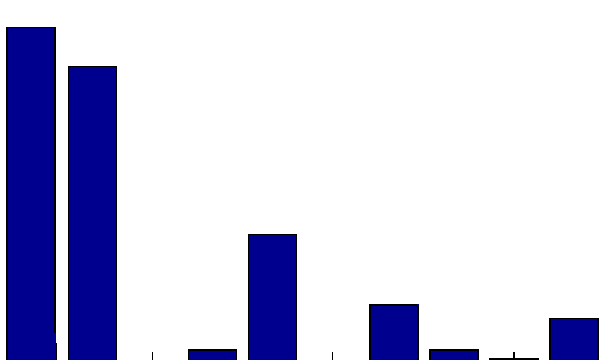
\includegraphics[width=0.225\textwidth, height=9mm]{bl5} &
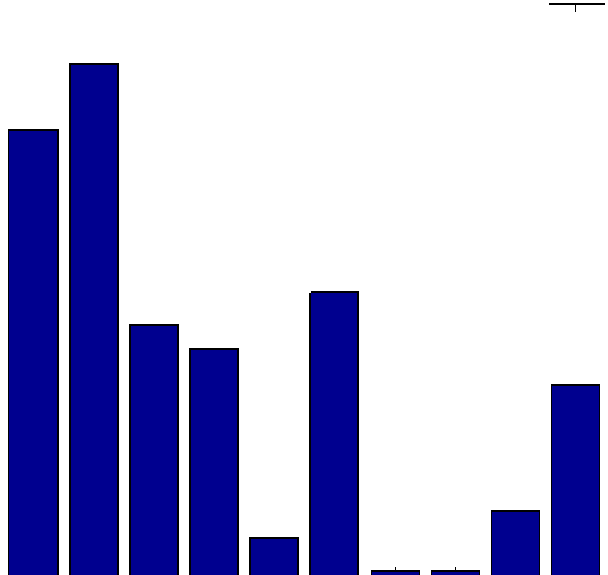
\includegraphics[width=0.225\textwidth, height=9mm]{bl6_2} &
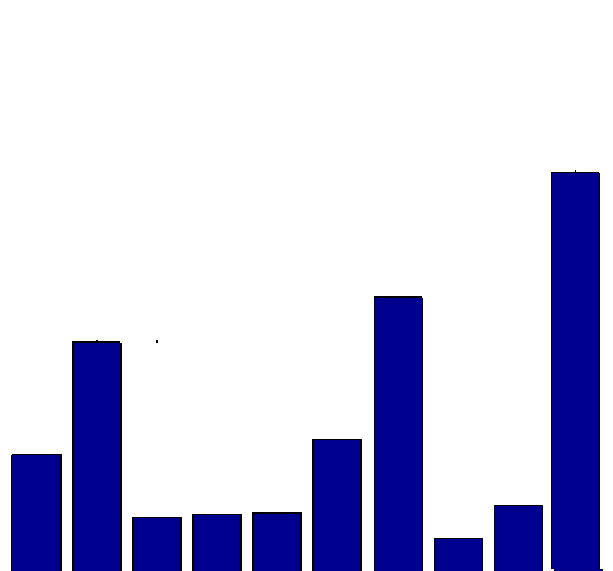
\includegraphics[width=0.225\textwidth, height=9mm]{bl7_2} &
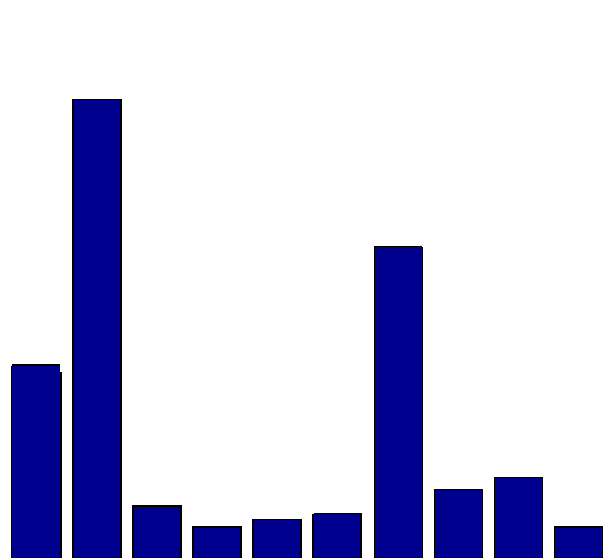
\includegraphics[width=0.225\textwidth, height=9mm]{bl8_2}  \\
\iffalse
\begin{tikzpicture}[remember picture,overlay]
\node[anchor=south west,inner sep=0] (image1)
  {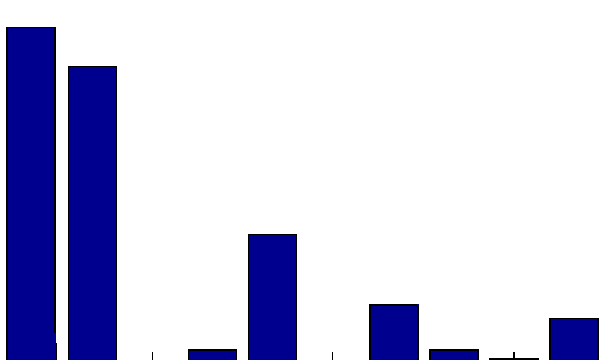
\includegraphics[width=0.22\textwidth, height=10mm]{bl5}};
\end{tikzpicture} &
\begin{tikzpicture}[remember picture,overlay]
\node[anchor=south west,inner sep=0] (image2)
  {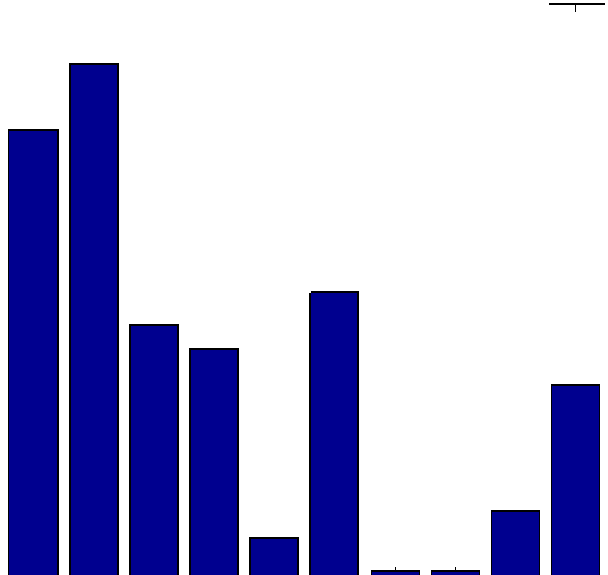
\includegraphics[width=0.22\textwidth, height=10mm]{bl6_2}};
\end{tikzpicture} &
\begin{tikzpicture}[remember picture,overlay]
\node[anchor=south west,inner sep=0] (image3)
  {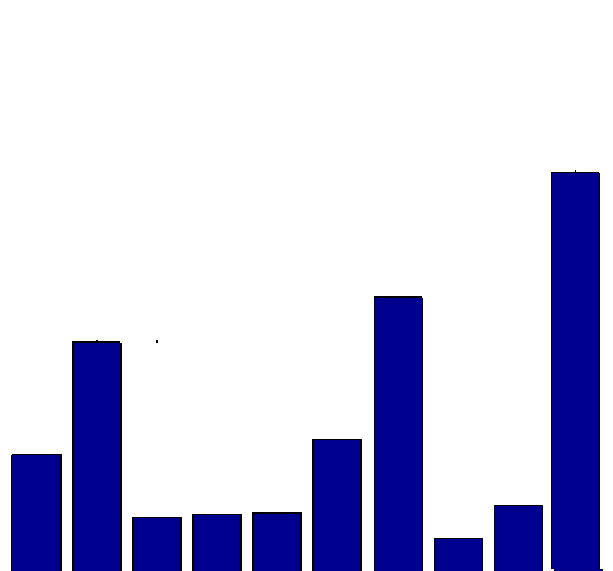
\includegraphics[width=0.22\textwidth, height=10mm]{bl7_2}};
\end{tikzpicture} &
\begin{tikzpicture}[remember picture,overlay]
\node[anchor=south west,inner sep=0] (image4)
  {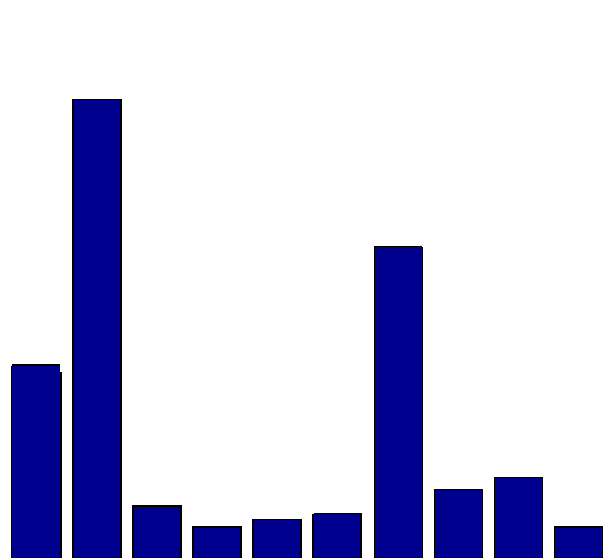
\includegraphics[width=0.22\textwidth, height=10mm]{bl8_2}};
\end{tikzpicture}
\begin{tikzpicture}[remember picture,overlay]
\draw[->,line width=2pt,red!80!black]
([yshift=-5pt,xshift=14pt]image4.west) |-
([yshift=-5pt,xshift=81pt]image3.west);
\draw[->,line width=2pt,red!80!black]
([yshift=0pt,xshift=81pt]image3.west) |-
([yshift=0pt,xshift=13pt]image2.west);
\draw[->,line width=2pt,red!80!black]
([yshift=-5pt,xshift=13pt]image2.west) |-
([yshift=-5pt,xshift=5pt]image1.west);
\end{tikzpicture}
\fi
\vspace{-6mm}\hspace{-1mm}\scalebox{0.84}{
\rotatebox[origin=r]{90}{reaching}\hspace{1mm}
\rotatebox[origin=r]{90}{moving}\hspace{1mm}
\rotatebox[origin=r]{90}{pouring}\hspace{1mm}
\rotatebox[origin=r]{90}{eating}\hspace{1mm}
\rotatebox[origin=r]{90}{drinking}\hspace{1mm}
\rotatebox[origin=r]{90}{opening}\hspace{1mm}
\rotatebox[origin=r]{90}{placing}\hspace{1mm}
\rotatebox[origin=r]{90}{closing}\hspace{1mm}
\rotatebox[origin=r]{90}{null}\hspace{1mm}
\rotatebox[origin=r]{90}{cleaning}}&
\vspace{-6mm}\hspace{-1mm}\scalebox{0.84}{
\rotatebox[origin=r]{90}{reaching}\hspace{1mm}
\rotatebox[origin=r]{90}{moving}\hspace{1mm}
\rotatebox[origin=r]{90}{pouring}\hspace{1mm}
\rotatebox[origin=r]{90}{eating}\hspace{1mm}
\rotatebox[origin=r]{90}{drinking}\hspace{1mm}
\rotatebox[origin=r]{90}{opening}\hspace{1mm}
\rotatebox[origin=r]{90}{placing}\hspace{1mm}
\rotatebox[origin=r]{90}{closing}\hspace{1mm}
\rotatebox[origin=r]{90}{null}\hspace{1mm}
\rotatebox[origin=r]{90}{cleaning}}&
\vspace{-6mm}\hspace{-1mm}\scalebox{0.84}{
\rotatebox[origin=r]{90}{reaching}\hspace{1mm}
\rotatebox[origin=r]{90}{moving}\hspace{1mm}
\rotatebox[origin=r]{90}{pouring}\hspace{1mm}
\rotatebox[origin=r]{90}{eating}\hspace{1mm}
\rotatebox[origin=r]{90}{drinking}\hspace{1mm}
\rotatebox[origin=r]{90}{opening}\hspace{1mm}
\rotatebox[origin=r]{90}{placing}\hspace{1mm}
\rotatebox[origin=r]{90}{closing}\hspace{1mm}
\rotatebox[origin=r]{90}{null}\hspace{1mm}
\rotatebox[origin=r]{90}{cleaning}}&
\vspace{-6mm}\hspace{-1mm}\scalebox{0.84}{
\rotatebox[origin=r]{90}{reaching}\hspace{1mm}
\rotatebox[origin=r]{90}{moving}\hspace{1mm}
\rotatebox[origin=r]{90}{pouring}\hspace{1mm}
\rotatebox[origin=r]{90}{eating}\hspace{1mm}
\rotatebox[origin=r]{90}{drinking}\hspace{1mm}
\rotatebox[origin=r]{90}{opening}\hspace{1mm}
\rotatebox[origin=r]{90}{placing}\hspace{1mm}
\rotatebox[origin=r]{90}{closing}\hspace{1mm}
\rotatebox[origin=r]{90}{null}\hspace{1mm}
\rotatebox[origin=r]{90}{cleaning}}
\end{tabular}
\end{tabular}
\caption{\textbf{Anticipated belief over activity.} In the first and third row, we show a middle frame of the temporal segment. In the second and fourth row, we show the anticipated belief we computed for the middle frame. Note that frames are not visible to the algorithm and only included for evaluation.}
%\vspace{-4mm}
\label{abcd}
%\end{singlespace}
\end{figure}


\noindent {\bf Data:} We use CAD-120 \cite{hemaIJRR} dataset in order to evaluate our method. CAD-120 dataset includes 120 RGB-D videos of four different subject performing activities \emph{reaching, moving, pouring, etc.} while interacting with objects having affordances \emph{reachable, movable, pourable, etc.}. There are 10 activity classes and 12 object affordance classes.

\noindent {\bf Experimental Setup:} For computing the features and learning the CRF parameters, we follow the approach and the code in \cite{hemaIJRR}. Following the convention in \cite{hemaIJRR}, we use 4-fold cross-validation by training over the data from 3 subjects and testing on the remaining subject. We then average the results over 4-folds. We implemented the rCRF as we explain in Algorithm~\ref{alg:recursive} with the following parameters obtainded via cross-validation; we sampled $M=15$ diverse samples and ran the recursive message updates with the number of iterations limit as $5$.

For the anticipation setting, In order to experiment the $\tau$ seconds into the future anticipation, we experiment over all feasible anticipation scenarios. In other words, we anticipated the time instant $t+\tau$ by using the segments $1\ldots t$ for all $t<T-\tau$, where $T$ is the length of the video. Then, we averaged the score over all feasible experiments.

\noindent {\bf Baseline Algorithms:} In detection setting, we compare the detection results of the rCRF to MAP solution of the spatiotemporal CRF in \cite{hemaIJRR}. We also included the state-of-the art activity detection results from Hu et al. \cite{latentIcra}. Moreover, \cite{latentIcra} is not based on object affordances and it only outputs activity detections. For the anticipation, we compare the rCRF with the state-of-the-art anticipation methods ATCRF \cite{hemaAnt} and GP-LCRF\cite{gpcrf}. We also include DCRF\cite{ddcrf}. In order to evaluate the contribution of the recursive modeling and the structured diversity separately, we also compare the rCRF with a recursive approach without diversity and a diversity-based approach without recursive modeling baselines.

The DivMBest algorithm in \cite{divmbest} uses the diverse sampling method to sample CRFs defined over each frame separately. DivMBest\cite{divmbest} then finds the most likely sequence via Viterbi algorithm. Since it is missing the recursive modeling, it serves as \emph{structured diversity without recursive filtering} baseline. We replace the diversity-based sampling in our method with Gibbs sampler and consider it as \emph{recursive filtering approach without structured diversity} baseline. For the Gibbs sampling, we sampled $50$ samples per temporal segment. We denote the recursive approach with Gibbs sampling as \emph{\mbox{"rCRF w/o div"}} while tabulating the results.

\noindent {\bf Evaluation Metrics:} For activity detection, we compute the ratio of the correctly classified labels (\emph{micro precision}) and the averages of the precision and recall values computed for each activity and object affordance classes (\emph{macro precision} and \emph{macro recall}). For anticipation, we record the ratio of the correctly classified labels \emph{micro precision}, the average of the f-1 score that is computed for each activity and object affordance class (\emph{macro f-1 score}), and the precision of the top 3 anticipated labels (\emph{robot anticipation metric}). While computing the \emph{robot anticipation metric}; if any of the top 3 anticipation is correct, it is counted as true positive.

\noindent {\bf Accuracy of the rCRF in detection setting.}
We evaluate the rCRF for activity detection and summarize the results in Table~\ref{Tdet}. Table~\ref{Tdet} suggests that the rCRF outperforms the MAP solution \cite{hemaIJRR} and performs similarly with the state-of-the-art solution \cite{latentIcra}. Since rCRF and \cite{hemaIJRR} are using the same spatial relations, the performance difference is due to the modeling of the temporal relations in rCRF. We use \mbox{first-order} statistics as temporal dynamics, and they are quite accurate as shown in the heatmap in Figure~\ref{heatmap}. They also capture semantic information like objects become stationary after being used.

\begin{figure}
  \subfigure[Human Activity]{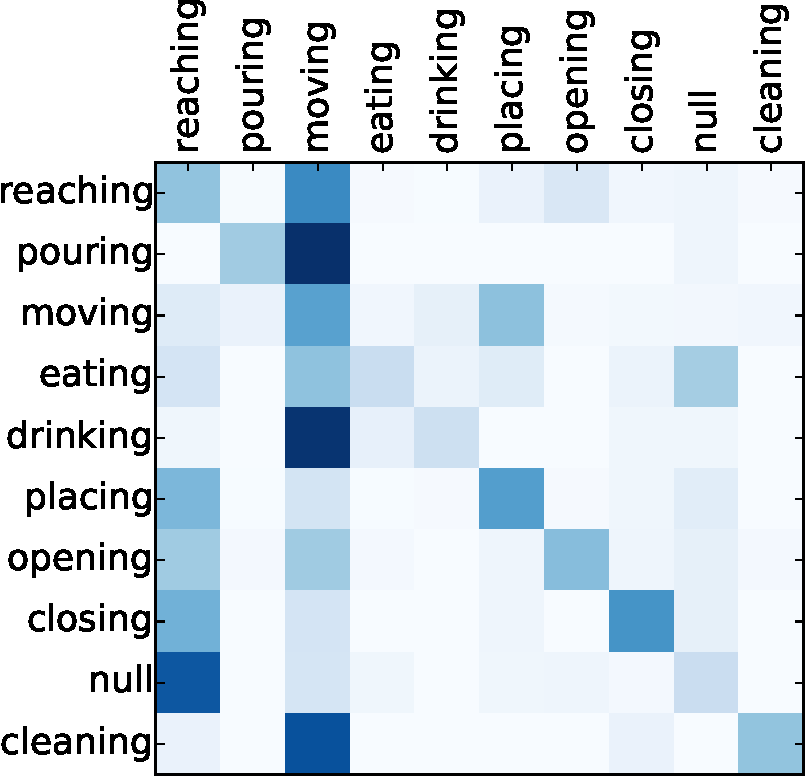
\includegraphics[width=0.48\textwidth]{tranAct}}~
  \subfigure[Object Affordance]{ 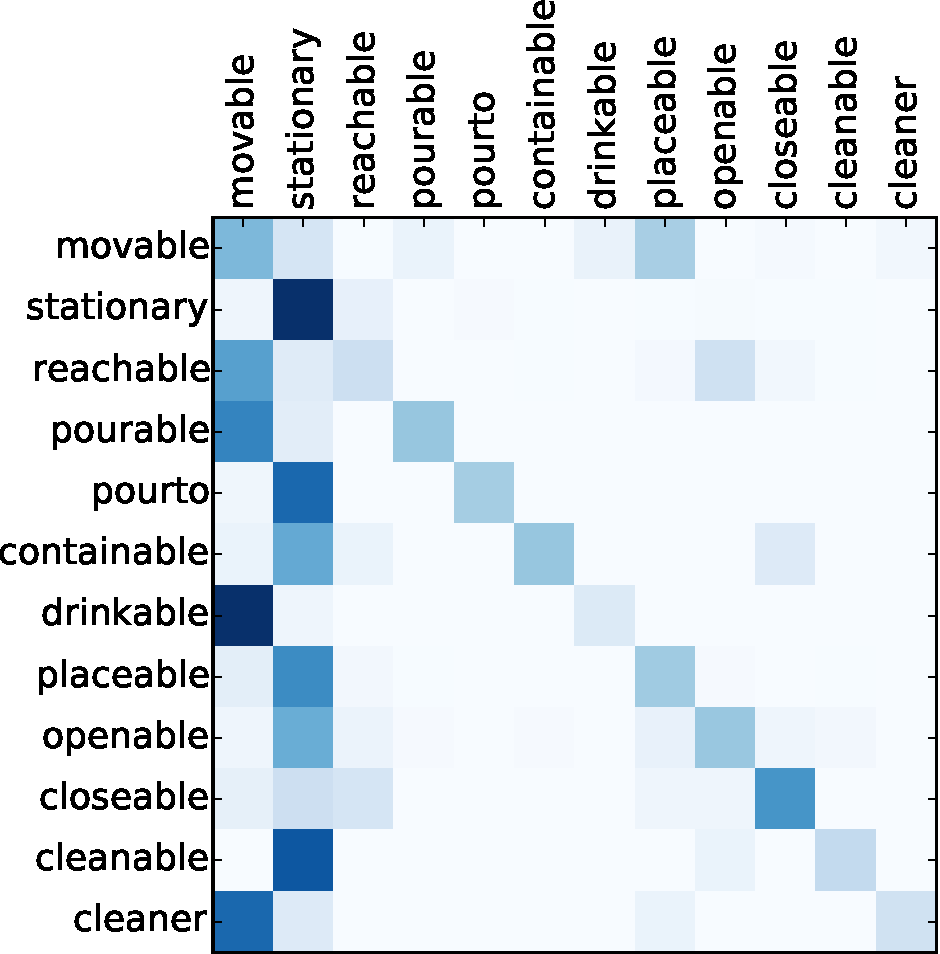
\includegraphics[width=0.48\textwidth]{tranObj}}
  \caption{Heatmap of the first-order statistics of activity and object affordance classes. They are used as temporal dynamics by rCRF.}
  \label{heatmap}
\end{figure}

\noindent {\bf Accuracy of the rCRF in anticipation setting.}
We evaluate the accuracy of the belief we compute via rCRF, both quantitatively and qualitatively. For qualitative evaluation, we show the segment that we are anticipating the belief over, as well as the belief we obtain in Figure~\ref{abcd}. Please note that, this visual information is not visible to the algorithm, and it is only included for the subjective evaluation.

As shown in the figure, anticipated belief is capturing the scene accurately. Belief is accurate even for the case of concurrent activities. For example, in the second column of the second row in Figure \ref{abcd}, subject is reaching the microwave and moving the cleaner. Our method assigns similar likelihood values to both reaching and moving.

We also perform quantitative analysis over anticipation accuracy. We anticipate 3 seconds into the future and summarize the results in Table~\ref{Tant}. As shown in the Table~\ref{Tant}, rCRF outperforms the state-of-the-art heuristic method \cite{hemaAnt} and the GP-LCRF method \cite{gpcrf} significantly as well as all other baselines. We believe this result is due to the accurate joint-modeling of the temporal relations and the CRF model. We further analysed this behaviour in the subsequent sections.

\begin{table}[ht]
\centering
\tabcolsep=0.7mm
\footnotesize
%\vspace{-1mm}
\caption{\textbf{Detection Performance over CAD-120.}  We compare rCRF with MAP solution and baselines for detections accuracy.}
%\vspace{-1mm}
\begin{tabular}{@{}l@{}|ccc|ccc@{}} \hline
& \multicolumn{3}{@{}|c@{}}{Sub-activity } &   \multicolumn{3}{@{}|c@{}}{Object Affordance } \\ \hline
& micro & \multicolumn{2}{@{}c|@{}}{macro} &   micro & \multicolumn{2}{@{}c@{}}{macro} \\
% \hline
 & prec(\%) & prec(\%) & rec(\%) &   prec(\%) & prec(\%) & rec(\%) \\
\hline
Chance & $10.0${\scriptsize $\pm 0.1$}  & $10.0${\scriptsize $\pm 0.1$}  & $10.0${\scriptsize $\pm 0.1$}  & $8.3${\scriptsize $\pm 0.1$}  & $8.3${\scriptsize $\pm 0.1$}  & $8.3${\scriptsize $\pm 0.1$}  \\
Hu et al.\cite{latentIcra} & $67.8${\scriptsize $\pm 1.4$}  &  $65.5${\scriptsize $\pm 3.5$}&  $\mathbf{63.5}${\scriptsize $\mathbf{\pm 6.6}$}  & N/A & N/A & N/A \\
MAP Sol\cite{hemaIJRR} & $63.4${\scriptsize $\pm 1.6$}  &  $65.3${\scriptsize $\pm 2.3$}&  $54.0${\scriptsize $\pm 4.6$}  & $79.4${\scriptsize $\pm 0.8$} & $62.5${\scriptsize $\pm 5.4$} & $50.2${\scriptsize $\pm 4.9$} \\
DivMBest\cite{divmbest}& $64.0${\scriptsize $\pm 1.3$} & $61.7${\scriptsize $\pm 2.1$} & $56.4${\scriptsize $\pm 2.7$} & $80.1${\scriptsize $\pm 1.0$} & $76.2${\scriptsize $\pm 2.5$} & $53.2${\scriptsize $\pm 3.2$} \\
DCRF\cite{ddcrf}& $61.2${\scriptsize $\pm 2.1$} & $62.8${\scriptsize $\pm 2.8$} & $54.3${\scriptsize $\pm 1.5$} & $71.9${\scriptsize $\pm 2.9$} & $80.6${\scriptsize $\pm 2.4$} & $62.5${\scriptsize $\pm 3.6$} \\
rCRF w/o div& $61.2${\scriptsize $\pm 1.8$} & $64.0${\scriptsize $\pm 1.8$} & $52.7${\scriptsize $\pm 3.8$} & $75.2${\scriptsize $\pm 2.4$} & $79.3${\scriptsize $\pm 3.1$} & $63.7${\scriptsize $\pm 2.9$} \\
rCRF&  $\mathbf{68.1}${\scriptsize$\mathbf{\pm 1.3}$} & $\mathbf{66.1}${\scriptsize $\mathbf{\pm 2.7}$} & $57.2${\scriptsize $\pm 3.9$} & $\mathbf{81.5}${\scriptsize $\mathbf{\pm 1.1}$} & $\mathbf{85.2}${\scriptsize $\mathbf{\pm 2.4}$} & $\mathbf{71.6}${\scriptsize $\mathbf{\pm 3.9}$} \\
\hline
\end{tabular}
%\end{singlespace}
\label{Tdet}
\end{table}
\begin{table}[ht]
\centering
\tabcolsep=0.7mm
\footnotesize
\vspace{-1mm}
\caption{\textbf{Anticipation performance for the anticipating 3 seconds in the future.} We compare rCRF with state-of-the-art anticipation algorithm and baselines for anticipation accuracy.}
\vspace{-1mm}
\begin{tabular}{@{}l@{}|ccc|ccc@{}} \hline
& \multicolumn{3}{@{}|c@{}}{Sub-activity } &   \multicolumn{3}{@{}|c@{}}{Object Affordance } \\ \hline
& micro & macro & robot ant. &  micro & macro & robot ant.   \\
Method & prec(\%) & f1-scr(\%) & metric(\%) & prec(\%) & f1-scr(\%) & metric(\%) \\ \hline
Chance & $10.0${\scriptsize $\pm 0.1$} & $10.0${\scriptsize $\pm 0.1$}  & $30.0${\scriptsize $\pm 0.1$} & $8.3${\scriptsize $\pm 0.1$} & $8.3${\scriptsize $\pm 0.1$}  & $24.9${\scriptsize $\pm 0.1$}  \\
GP-LCRF \cite{gpcrf} & $52.1${\scriptsize $\pm 1.2$} & $43.2${\scriptsize $\pm 1.5$} &  $76.1${\scriptsize $\pm 1.5$}  & $68.1${\scriptsize$\pm 1.0$}  & $44.2${\scriptsize $\pm 1.2$}  & $74.9${\scriptsize $\pm 1.1$}  \\
ATCRF \cite{hemaAnt} & $47.7${\scriptsize $\pm 1.6$} & $37.9${\scriptsize $\pm 2.6$} &  $69.2${\scriptsize $\pm 2.1$}  & $66.1${\scriptsize $\pm 1.9$}  & $36.7 ${\scriptsize $\pm 2.3$}  & $71.3${\scriptsize $\pm 1.7$}  \\
DivMBest\cite{divmbest}& $47.9${\scriptsize $\pm 1.4$} & $43.2${\scriptsize $\pm 3.6$} & $71.5${\scriptsize $\pm 2.7$} & $61.3${\scriptsize $\pm 1.4$} & $56.3 ${\scriptsize $\pm 2.1$} & $73.3${\scriptsize $\pm 0.5$} \\
DCRF\cite{ddcrf}& $48.3${\scriptsize $\pm 2.6$} & $35.4${\scriptsize $\pm 1.8$} & $66.6${\scriptsize $\pm 1.1$} &
$55.2${\scriptsize $\pm 3.1$} & $48.5${\scriptsize $\pm 3.1$} & $71.24${\scriptsize $\pm 2.2$} \\
rCRF w/o div& $49.6${\scriptsize $\pm 2.1$} & $39.7${\scriptsize $\pm 2.6$} & $65.1${\scriptsize $\pm 1.1$} & $56.2${\scriptsize $\pm 1.9$} & $47.4${\scriptsize $\pm 3.1$} & $70.8${\scriptsize $\pm 2.5$} \\
rCRF & $\mathbf{54.3}${\scriptsize $\mathbf{\pm 3.9}$} & $\mathbf{45.8}${\scriptsize $\mathbf{\pm 2.7}$} & $\mathbf{76.5}${\scriptsize $\mathbf{\pm 2.6 }$}  & $\mathbf{78.7}${\scriptsize $\mathbf{\pm 3.4}$} &$\mathbf{74.9}${\scriptsize $\mathbf{\pm 3.8}$} & $\mathbf{82.1}${\scriptsize $\mathbf{\pm 2.9}$} \\
\hline
\end{tabular}
\label{Tant}
\end{table}

\noindent {\bf How important is the recursive modeling?}
DivMBest\cite{divmbest} is the application of the structured diversity without recursive modeling of the Bayesian filtering. In all experiments (Table~\ref{Tdet} and \ref{Tant}), rCRF outperforms the DivMBest \cite{divmbest}. We believe this is because rCRF samples  $p(y^t|x^1,\ldots,x^T)$ instead of $p(y^t|x^t)$ as in the case of \cite{divmbest}. In other words, DivMBest \cite{divmbest} samples without considering temporal relations; on the contrary, we sample the full belief directly.

Moreover, the improvement over the DCRF model shows the important of accurate recursive modeling. DCRF uses the recursive modeling without the proposed conversion of the discrimantive likelihood into generative one and it performs poorly. Hence, the proposed conversion is a necessary step.

We also studied the effect of anticipation horizon. We computed precision of all methods for horizons between 1 and 10 seconds and plotted in Figure~\ref{antHor} and \ref{objHor}. We see significant improvements over longer anticipation time horizons.%\footnote{Since ATCRF \cite{hemaAnt} and GP-LCRF \cite{gpcrf} are using the same method to anticipate the future activities and they only differ in modeling details of humans, they behave similarly versus anticipation time as shown in \cite{gpcrf} and we only included \cite{hemaAnt} in the plot.}
%  and we only included \cite{hemaAnt} in the plot for the sake of clarity.
%We only show the result on object affordance anticipation and rest of the results are included in the supplementary material.

In Figure~\ref{antHor} and \ref{objHor}, accuracy of all algorithms decreases with the increasing horizon. One interesting observation is decrease rate of DivMBest is steeper than others. Since DivMBest misses the recursive nature of the problem, accuracy of the belief it computes is limited; hence, the resulting belief does not stay informative with increasing horizon.

\begin{figure}[ht]
\begin{center}
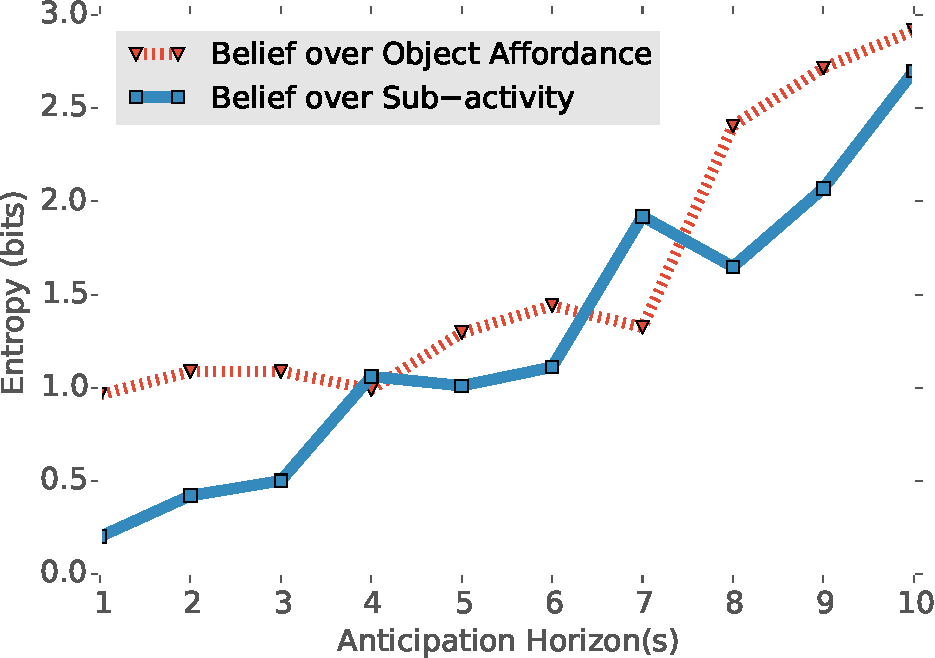
\includegraphics[width=\textwidth]{entTwo}
\caption{Entropy of the belief vs. time \emph{(uniform dist. has $\approx 3.32$ bit entropy)}}
\label{entRop}
\end{center}
\end{figure}

We further computed the entropy of the belief rCRF computes and plotted its average in Figure~\ref{entRop}. The decrease rate of the accuracy is much smaller than the increase rate of the entropy. In summary, recursive modeling is necessary for an accurate belief estimation and rCRF computes flatter yet still informative beliefs with increasing horizon.

\noindent {\bf How to efficiently cover the output space?}
In order to see the effect of structural diversity on covering the output space, we compare the rCRF with a version of it in which we replace diverse sampling with the Gibbs sampler. As expected, Gibbs sampler only sampled the small region around the posterior and failed to cover the output space. Within all experiments, rCRF outperforms Gibbs sampler baseline. Another interesting observation is, as shown in Figure~\ref{antHor}\&\ref{objHor}, although Gibbs sampler based method performed slightly better than other baselines for short horizon activity anticipation, it performed much worse for object affordance. We believe this is because of the dimensionality. Activity space has dimension $10^{T}$ whereas the object affordance space has dimension $12^{T\cdot M}$ where $T$ is the length of the video and $M$ is the number of objects. Hence, diversity plays bigger role with increasing dimension. Moreover, \cite{hemaAnt} uses the domain knowledge by selectively sampling points around the hand, etc. and it performs better than both baselines with increasing horizon. We believe this result is due to the efficient coverage of the output space with heuristics.

\begin{figure}[t]
  \centering
  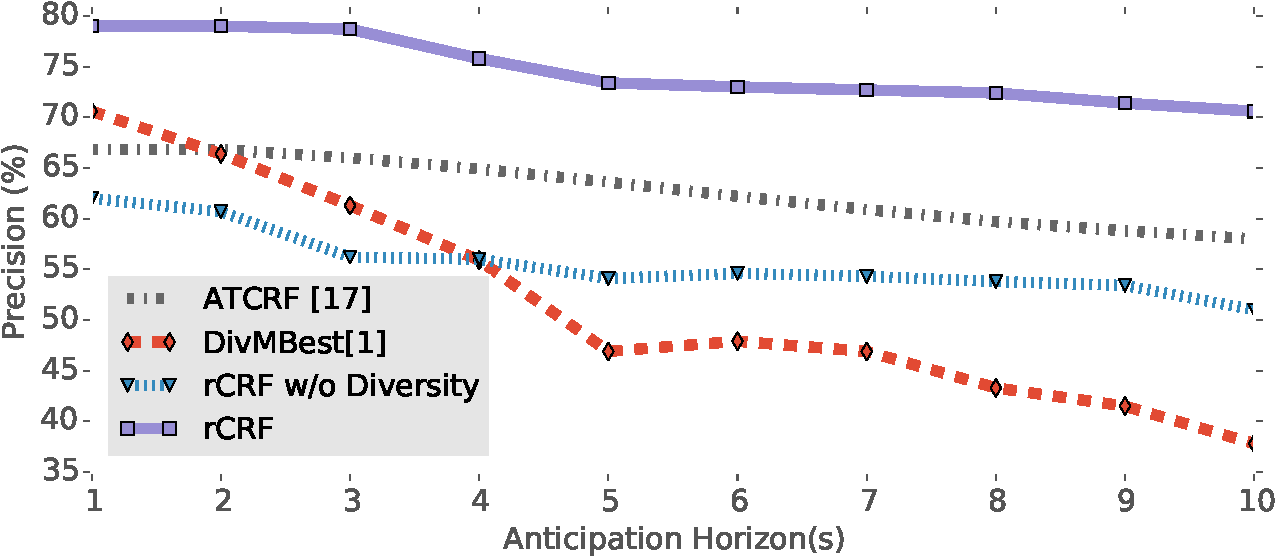
\includegraphics[width= \textwidth]{AntO}
\caption{Precision vs. anticipation horizon for object affordance.}
\label{antHor}
\end{figure}

\begin{figure}[h!]
  \centering
  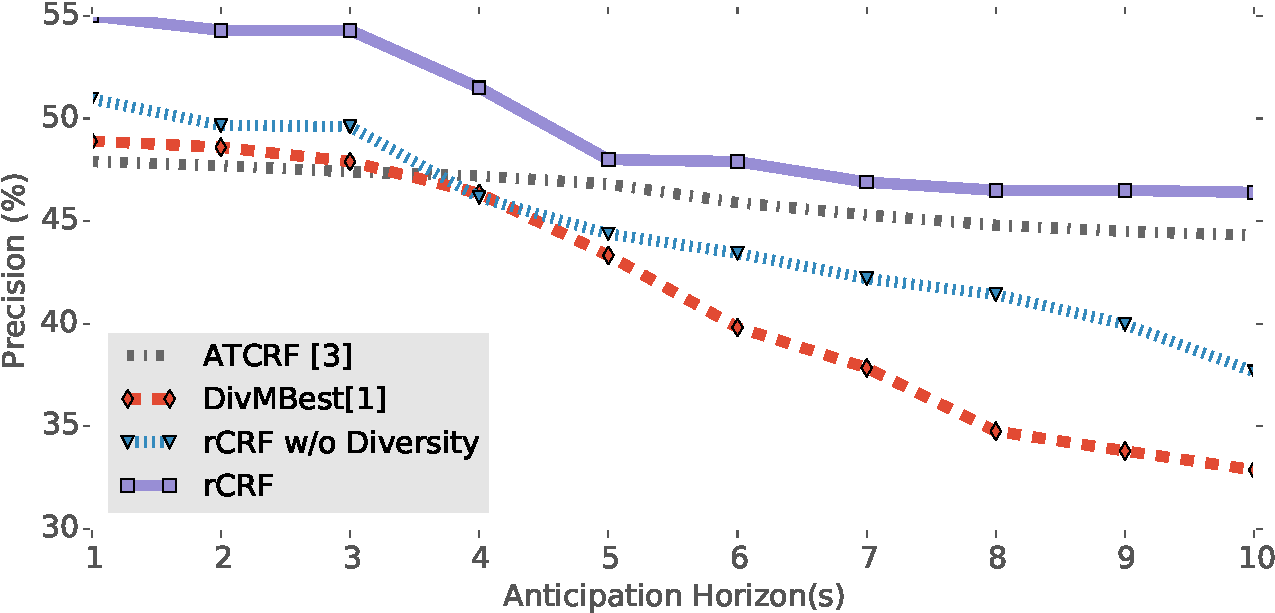
\includegraphics[width=\textwidth]{AntA}
\caption{Precision vs. anticipation horizon for subject activities.}
\label{objHor}
\end{figure}

\noindent {\bf Computationally-efficient inference:}
We evaluated the computational efficiency by computing the average computation time for anticipating 3 second in the future via rCRF and the fastest available anticipation algorithm (the ATCRF\cite{hemaAnt}). Within our experiments, we did not include any pre-processing or feature extraction computation (they are same for all algorithms). Our experiments suggest that the rCRF is faster than \cite{hemaAnt} as shown in Table~\ref{speed}. Hence, rCRF model outperforms the state-of-the-art anticipation algorithm in terms of speed in addition to the accuracy.
\begin{table}[h!]
  \centering
%  \vspace{-2mm}
\caption{Computation time for anticipating 3 seconds in the future excluding pre-processing (\emph{see supplementary material for details}).}
%\vspace{-2mm}
  \begin{tabular}{|cc|cc|}
    \hline
  ATCRF \cite{hemaAnt} \; \; & \; \; 34.1s  \; \;  \; & \; \; \;  rCRF \; \; & \; \;  1.41s \\ \hline
  \end{tabular}
  \vspace{-1mm}
  \label{speed}
\end{table}
%\vspace{-2mm}

\noindent {\bf Can rCRF generalize to RGB data?:}
Since there is no RGB activity dataset with object labels, it is hard to compare our algorithm in the RGB activity analysis setting. Removing the concept of the objet form the graph, makes it a chain-CRF and the inference and learning becomes straightforward. However, we still implement our rCRF over a linear-chain CRF for RGB activity analysis. We based our implementation on MPII cooking activity dataset \cite{mpi_cooking} and use the publicly distributed features from the authors webpage. The shared features are HOG, HOF, dense trajetory features and  MBH \cite{dalal}.


%\begin{table}
\begin{table}
  \caption{Anticipation performance for the anticipating 3 seconds in the future in MPII Cooking Dataset\cite{mpi_cooking}.}
\begin{tabular}{l|ccc} \hline
& micro & macro & macro  \\
Method & prec(\%) & prec(\%) & recall(\%) \\ \hline
Chance & $1.5${\scriptsize $\pm 0.6$} & $1.5${\scriptsize $\pm 0.6$}  & $1.5${\scriptsize $\pm 0.6$}  \\
ATCRF \cite{hemaAnt} & $33.4${\scriptsize $\pm 3.3$} & $52.1${\scriptsize $\pm 4.6$}  & $12.1${\scriptsize $\pm 1.4$}  \\
DivMBest\cite{divmbest} & $34.4${\scriptsize $\pm 2.8$} & $55.3${\scriptsize $\pm 5.0$}  & $14.3${\scriptsize $\pm 1.2$}  \\
rCRF & $\mathbf{37.4}${\scriptsize $\mathbf{\pm 2.9}$} & $\mathbf{63.2}${\scriptsize $\mathbf{\pm 5.5}$}  & $\mathbf{26.1}${\scriptsize $\mathbf{\pm 2.6}$}  \\
\hline
\end{tabular}
\label{Tantmpi}
\end{table}

As shown in the Table~\ref{Tantmpi}, our method outperforms all baselines and competing algorithms. We did not include Gibbs sampling here since the dimension of the activity space is rather low and the experiment over diversity is not informative. We believe this result is due to the accurate handling of temporal information in rCRF and it shows that it generalizes to other modalities.


% !TEX root = rCRF.tex

\section{Conclusions}

In this work, we consider the problem of using rich \mbox{CRF-based} scene models in Bayesian filtering setting. We presented the rCRF model which uses rich modelling power of CRFs in recursive Bayesian filtering. We further developed a computationally-tractable method based on Jensen inequality and structured diversity. We performed extensive experiments that
%  the proposed method against the state-of-the-art methods and various baselines. We 
show rCRF  accurately anticipates the future beliefs over CRFs. We also experimentally demonstrated that the recursive framework significantly improves the accuracy of anticipation. Our rCRF not only resulted in more accurate anticipation but also improved the computation time.   


\vspace{5mm}

\noindent\textbf{Acknowledgement.} We thank Hema Koppula for helpful discussions. This research was funded in part by Microsoft
Faculty Fellowship (to Saxena), NSF Career award (to
Saxena) and Army Research Office.

% \clearpage
{
\small
\bibliography{shortstrings,anticipation_divmrf}
\bibliographystyle{plainnat}
}

\end{document}
